\documentclass[10pt,a4paper]{article}

\usepackage[a4paper,margin=2.55cm]{geometry}
\usepackage[T1]{fontenc}
\usepackage[utf8]{inputenc}
\usepackage{lmodern}
\usepackage{microtype}
\usepackage{graphicx}
\usepackage{booktabs}
\usepackage{array}
\usepackage{longtable}
\usepackage{tabularx}
\usepackage{float}
\usepackage{caption}
\usepackage{subcaption}
\usepackage{xcolor}
\usepackage{enumitem}
\usepackage{amsmath}
\usepackage[hidelinks]{hyperref}
\usepackage{placeins}

\graphicspath{{../../results/}{../../specification/}{../img/}}
\hypersetup{
    pdftitle={Wind-Assisted Propulsion on North Sea Routes},
    pdfauthor={Aleksandra Klos, Olga Grigorieva, Elen Mouradian, Bartosz Maj, Hubert Jaczynski},
    pdfsubject={Maritime performance analytics for Flettner rotors},
    pdfkeywords={wind-assisted propulsion, Flettner rotors, AIS, ERA5, Copernicus Marine, maritime analytics}
}

\setlength{\parskip}{0.38em}
\setlength{\parindent}{0pt}
\emergencystretch=3em
\setlist[itemize]{leftmargin=1.35em,itemsep=0.2em,topsep=0.2em}
\setlist[enumerate]{leftmargin=1.45em,itemsep=0.2em,topsep=0.2em}
\captionsetup{font=small,labelfont=bf}

\newcommand{\kn}{\ensuremath{\mathrm{kn}}}
\newcommand{\ms}{\ensuremath{\mathrm{m/s}}}
\newcommand{\kw}{\ensuremath{\mathrm{kW}}}
\newcommand{\co}{CO$_2$}
\newcommand{\hs}{$H_s$}
\newcommand{\sog}{SOG}
\newcommand{\cog}{COG}
\newcommand{\alphaabs}{$|\alpha|$}

\title{\textbf{Wind-Assisted Propulsion on North Sea Routes}\\
\large Maritime Performance Analytics for Flettner Rotors}
\author{Aleksandra K\l{}os \and Olga Grigorieva \and Elen Mouradian \and Bartosz Maj \and Hubert Jaczy\'nski}
\date{DataWaves Innovation Laboratory \\
Conference submission, May 2026}

\begin{document}
\pagenumbering{gobble}

\begin{titlepage}
    \centering
    \vspace*{1.2cm}
    {\Huge\bfseries Wind-Assisted Propulsion on North Sea Routes\par}
    \vspace{0.35cm}
    {\Large Maritime Performance Analytics for Flettner Rotors\par}
    \vspace{0.9cm}
    {\large DataWaves Innovation Laboratory -- Conference submission\par}
    \vspace{0.25cm}
    {\large May 2026\par}
    \vspace{1.2cm}
    {\large
    Aleksandra K\l{}os\\
    Olga Grigorieva\\
    Elen Mouradian\\
    Bartosz Maj\\
    Hubert Jaczy\'nski\par}
\end{titlepage}

\pagenumbering{arabic}
\tableofcontents
\clearpage

\section{Executive summary}

The project studies how wind, waves, currents, and vessel heading influence
operational speed on North Sea routes, and whether Flettner rotors can improve
voyage performance or enlarge useful weather windows. The work follows the
advanced study brief: AIS position reports were merged with ERA5
wind fields and Copernicus Marine sea-state/current variables
\cite{hersbach2020era5,copernicusmarine}, transformed into trajectory-aware
features, modelled with leakage-aware train/test splits, and used in a
rotor-assisted what-if simulation.

The final engineered dataset contains 125,160 AIS-metocean observations from
528 voyages between 2023-02-02 and 2026-02-02. The speed target is
\sog{} in knots. The modelling split is chronological by voyage: 422 voyages
and 88,346 rows are used for training; 106 later voyages and 35,758 rows are
held out for testing. This design prevents observations from the same voyage
from appearing on both sides of the split and avoids temporal leakage.

Four model levels were evaluated. A constant-speed baseline gives MAE
1.388 \kn{} and RMSE 1.893 \kn{}. A linear model using wind, wave height, and
encoded wind angle gives a small improvement, MAE 1.377 \kn{} and $R^2=0.034$.
A weather-only XGBoost model is useful for interpretation but does not improve
test accuracy under the current feature set. The best predictive model is the
lagged nowcast XGBoost model, which adds previous observed \sog{} and apparent
wind context; it reaches MAE 0.406 \kn{}, RMSE 0.758 \kn{}, $R^2=0.839$, and
91.7\% of predictions within $\pm 1$ \kn{}.

The rotor scenario is deliberately applied after prediction rather than used as
a training feature. Rotor power is estimated from the provided polar diagram and
converted to a speed increment with the scenario assumption
200 \kw{} $\approx$ 1 \kn{} near the operating point. On the held-out test set,
the rotor is active in 98.1\% of observations, with mean active rotor power
41.2 \kw{}, mean active speed contribution 0.206 \kn{}, and overall mean
contribution 0.202 \kn{}. Under the weather-window definition
\sog{} $\geq 10$ \kn{} and \hs{} $\leq 3$ m, coverage increases from 76.0\% in
the baseline prediction to 77.5\% after adding the rotor scenario. The number
of separate windows decreases from 866 to 808, while points inside windows
increase by 529, suggesting that some marginal windows become longer and merge
when rotor assistance is applied.

Because the historical AIS period may already include rotor-assisted operation,
the scenario should be read as a transparent rotor-opportunity estimate rather
than as a measured causal before/after effect.

The optional extensions add operational interpretation. The energy model
estimates 112.2 t of fuel saved and 349.4 t \co{} avoided over the three-year
dataset, or about 37.4 t fuel and 116.4 t \co{} per year. Route segmentation
shows different benefits by heading regime, with westbound legs gaining the
largest weather-window coverage increase. Route optimisation demonstrates a
Dijkstra grid-routing proof of concept for rotor gain. Gain detection shows that
only 11.9\% of observations are high-gain moments, but those moments carry a
large share of the total benefit; high gain is associated mainly with wind
speeds above 8--12 \ms{} and beam-to-quartering apparent wind angles.

\begin{table}[H]
\centering
\caption{Main quantitative outcomes from the analysis run.}
\begin{tabularx}{\textwidth}{>{\raggedright\arraybackslash}p{0.33\textwidth}X}
\toprule
\textbf{Area} & \textbf{Current result} \\
\midrule
Dataset & 125,160 observations, 528 voyages, 2023-02-02 to 2026-02-02. \\
Validation & Chronological voyage split; 422 train voyages and 106 test voyages; no temporal leakage. \\
Best speed model & XGBoost lagged nowcast: MAE 0.406 \kn{}, RMSE 0.758 \kn{}, $R^2=0.839$. \\
Rotor speed uplift & Mean active $\Delta$\sog{} 0.206 \kn{}; overall mean $\Delta$\sog{} 0.202 \kn{}. \\
Weather windows & Coverage 76.0\% for the baseline prediction and 77.5\% after adding the rotor scenario; +529 test observations inside windows. \\
Fuel and emissions & Scenario estimate of 112.2 t fuel saved and 349.4 t \co{} avoided over the dataset; annualised 37.4 t fuel and 116.4 t \co{}. \\
High-gain moments & 11.9\% of observations have $\Delta$\sog{} $\geq 0.5$ \kn{}; classifier F1 = 0.992. \\
\bottomrule
\end{tabularx}
\end{table}

\section{Project context and objectives}

Commercial vessels increasingly use wind-assisted propulsion to reduce fuel
burn, emissions, and exposure to volatile fuel prices. A Flettner rotor is a
rotating vertical cylinder. When wind flows around it, the Magnus effect creates
an aerodynamic lift force. Depending on the apparent wind angle and the vessel's
course, part of this force can point forward and support the main engine. In
practice the contribution is highly conditional: the same rotor can be useful,
neutral, or even unfavourable depending on wind speed, angle, sea state, vessel
speed, and operational constraints. This conditionality is consistent with
published route-based and ship-performance studies of Flettner rotors and other
wind-assisted propulsion technologies \cite{traut2014flettner,lu2020wasp}.

The study brief defines the problem as an algorithmic analysis of vessel traces
and metocean conditions. The expected outputs are dependencies between
environmental conditions and voyage parameters, a scenario comparison between
baseline and rotor-assisted operation, and an assessment of weather windows for
sailing. The advanced version asks for current/tide vectors, apparent wind
calculation, rotor modelling, weather-window estimation, and uncertainty
analysis. The analysis implements each of these elements.

The practical goal is not to build a final naval-architecture simulator. Instead,
the goal is to create a transparent decision-support prototype that can answer
questions such as:

\begin{itemize}
    \item How accurately can \sog{} be predicted from forecast-available
    metocean variables and recent vessel behaviour?
    \item Which environmental variables appear to influence speed under the
    current data and modelling setup?
    \item Under what wind-speed and wind-angle combinations do rotors provide
    meaningful operational gain?
    \item Do rotors increase the fraction of time in which a voyage satisfies a
    useful weather-window criterion?
    \item Can energy, \co{}, route segmentation, and routing analyses be built
    consistently on top of the same feature set?
\end{itemize}

This framing is important because wind-assisted propulsion is not a single
constant correction to vessel speed. A rotor does not simply add the same
number of knots in all conditions. It depends on the direction and strength of
the wind seen by the ship, the ship's course, the current, and the operational
state of the vessel. A model that ignores those dependencies may still produce a
number, but it would not be useful for route planning or for deciding when the
rotor is actually valuable.

The wider motivation is also regulatory and environmental. The IMO greenhouse
gas studies identify international shipping as a material source of global
emissions and provide a common reference point for evidence-based reduction
measures \cite{imo2020ghg}.

The project therefore treats the problem as a chain of decisions. First, the
trajectory has to be reconstructed and enriched with environmental context.
Second, speed has to be predicted in a way that respects voyages and time.
Third, a rotor scenario has to be applied consistently to the same observations.
Finally, the result has to be translated into operational quantities: weather
windows, fuel, \co{}, route segments, and high-gain moments. Each stage is
deliberately kept visible in the notebooks so that a reviewer can see where the
numbers come from.

There is also an interpretability goal. A purely black-box result such as
``rotors improve performance'' would not be enough for a maritime user. The
operator needs to know when the improvement appears, what assumptions created
it, and whether the result is stable enough to support planning. For that
reason the report separates predictive accuracy from physical interpretation.
The lagged model answers a practical nowcasting question. The weather-only and
rotor-gain analyses answer a different question: what environmental structure
is associated with better or worse performance?

\subsection{Operational meaning of the problem}

The operational problem can be described from the perspective of a voyage
planner. Before a voyage, the planner has a forecast of wind, waves, and
currents, a desired route, and a schedule. During the voyage, the operator also
has recent vessel speed and a clearer view of how the ship is behaving. The
project supports both moments. The weather-only features are closer to the
pre-voyage planning situation, while the lagged nowcast model is closer to an
in-voyage monitoring situation.

Weather windows are a natural way to turn model output into an operational
language. A ship does not only need a high average speed; it needs continuous
periods in which speed and sea state are acceptable. A short improvement may be
irrelevant if it happens during an already safe and fast period. A small speed
increase may be valuable if it connects two otherwise separated windows, keeps a
voyage above a schedule threshold, or allows the main engine to run at a lower
load while preserving the same arrival time.

This is why the report tracks both speed-prediction metrics and window metrics.
Regression metrics show whether the model can reproduce observed speed.
Window metrics show whether the predicted difference changes the operational
classification of a route segment. The two are related but not identical. A
model can have a modest average speed improvement and still be useful if the
improvement occurs at the threshold where decisions are made.

\subsection{Key concepts}

Several terms appear repeatedly in the report. \sog{} means speed over ground:
the speed of the vessel relative to the Earth, including the effect of current.
\cog{} means course over ground: the direction in which the vessel is moving on
the map. These are AIS-derived movement quantities, not direct measurements of
engine load or speed through water.

\begin{table}[H]
\centering
\caption{Short glossary for the main operational and modelling concepts.}
\begin{tabularx}{\textwidth}{>{\raggedright\arraybackslash}p{0.25\textwidth}X}
\toprule
\textbf{Concept} & \textbf{Meaning in this project} \\
\midrule
\sog{} & Observed or predicted vessel speed over ground, measured in knots. \\
\cog{} & Vessel movement direction over ground, used to define route context and relative angles. \\
\hs{} & Significant wave height, used both as a sea-state feature and as part of the weather-window threshold. \\
True wind & Wind from the gridded metocean product, before correcting for vessel motion. \\
Apparent wind & Wind experienced by the moving vessel; especially important for rotor behaviour. \\
Relative wind angle & Angle between wind direction and vessel course; one of the main drivers of rotor usefulness. \\
Weather window & A continuous period where the predicted speed and wave state satisfy an operational threshold. \\
High-gain moment & An observation where the rotor scenario gives a speed contribution of at least 0.5 \kn{}. \\
\bottomrule
\end{tabularx}
\end{table}

This terminology also explains why the project uses vector and angle features
instead of only scalar wind and wave values. A wind speed of 10 \ms{} can be
helpful, neutral, or unfavourable depending on its direction relative to the
ship. A current of the same magnitude can support the ship, oppose it, or push
it sideways. The model therefore needs both magnitudes and directions to
represent maritime performance in a way that is useful for decision-making.


\section{Data sources and preprocessing}

\subsection{Raw inputs}

The core input is a set of AIS-derived position reports for the analysed vessel.
Each point contains time, latitude, longitude, speed over ground, course over
ground, and trajectory-derived distance fields. These observations are enriched
with gridded metocean data from numerical models:

\begin{itemize}
    \item ERA5 wind variables: 10 m wind components and gust information.
    \item Copernicus Marine sea state: significant wave height, mean wave
    direction, and mean wave period.
    \item Copernicus Marine currents: eastward and northward current components.
\end{itemize}

AIS is used here as a standardised vessel movement trace; the technical
characteristics of the underlying VHF automatic identification system are
defined by ITU-R Recommendation M.1371 \cite{itu2026ais}. The environmental
context follows established reanalysis and operational ocean-data sources:
ERA5 for atmospheric fields \cite{hersbach2020era5} and Copernicus Marine for
marine waves and currents \cite{copernicusmarine}.

The merged \texttt{MasterSet.csv} file contains the base AIS-metocean table.
The engineered feature file contains the modelling
features used by the baseline and extension notebooks. The feature-engineering
notebook reports 125,160 rows and 57 columns after processing.

AIS data should be interpreted as an operational trace rather than a laboratory
measurement. It tells us where the vessel was and how fast it moved over the
ground, but it does not fully explain why it moved that way. Speed can be
affected by engine settings, safety margins, traffic, port approach rules,
cargo state, draught, fouling, and schedule decisions. Some of those factors are
not present in the dataset. This is the main reason the project keeps a simple
constant-speed baseline and a linear weather baseline in the evaluation: they
show how much the more complex models improve over a minimal explanation.

The environmental data provide the surrounding physical context. ERA5 wind
fields are used to describe the air flow that drives the rotor scenario and
affects resistance. Copernicus wave variables describe sea-state severity, which
is important because high waves can reduce speed or make a route operationally
unattractive even if the wind is favourable. Current vectors are included
because the target is speed over ground. A following current and an opposing
current can change observed ground speed even if the vessel's speed through the
water is similar.

The final modelling table is therefore a joined view of two different worlds:
the ship trajectory and the gridded environment. The value of the table comes
from the fact that every row is an interpretable event: at this time, in this
position, on this voyage, the vessel had this course and speed, while the
surrounding wind, wave, and current conditions had these values.

\subsection{Spatio-temporal alignment}

AIS points are irregular in time and space, while metocean products are gridded.
The preprocessing pipeline aligns these sources by interpolating environmental
variables to each AIS position and timestamp. This is the key step that turns a
vessel trajectory into a supervised learning table. For each AIS observation the
pipeline attaches the environmental state that the vessel experienced at that
location and time.

The workflow separates this work across proof-of-concept interpolation,
ERA5-checking, exploratory-analysis, and feature-engineering notebooks. The
resulting dataset spans 2023-02-02 to 2026-02-02 and covers 528 voyages.

The alignment step is especially important for wind-assisted propulsion. A
small time mismatch can change the estimated wind angle, and a spatial mismatch
can attach weather from the wrong grid cell. For ordinary exploratory analysis,
that error may only add noise. For rotor analysis, it can change whether an
observation is classified as favourable or unfavourable. This is because rotor
power is strongly directional: the difference between near-beam wind and
near-headwind can be the difference between positive useful power and almost no
benefit.

The project also treats voyages as groups rather than as a single continuous
stream. This avoids mixing different trips and prevents lag features from
borrowing information across voyage boundaries. It also makes evaluation more
realistic. A future voyage is not just another random row from the same trip; it
is a new sequence of points with its own route, season, weather, and operating
pattern.

\begin{figure}[H]
    \centering
    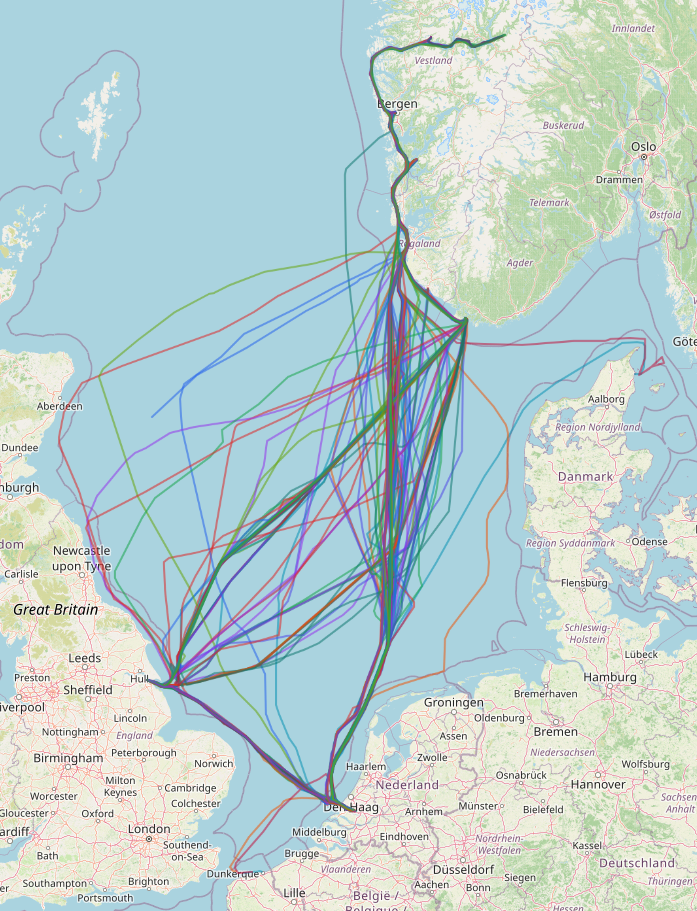
\includegraphics[width=0.88\textwidth]{all_trajectories_osm.png}
    \caption{Training trajectories used by the project pipeline, shown on an
    OpenStreetMap basemap for geographic context \cite{osm}.}
\end{figure}

\subsection{Feature engineering}

The engineered variables follow a leakage-aware design. Features are divided
into explanatory metocean/route variables, lagged nowcast variables, and
post-prediction rotor-scenario variables. The main feature groups are:

\begin{itemize}
    \item \textbf{Wind and wave features}: true wind speed, significant wave
    height \hs{}, wave period, wind speed squared, and wave-wind alignment.
    \item \textbf{Relative-angle features}: wind direction and angle relative to
    vessel course, encoded with sine/cosine terms to avoid discontinuity at
    0/360 degrees.
    \item \textbf{Apparent wind features}: apparent wind speed and apparent
    relative angle, reserved for the nowcast model.
    \item \textbf{Current features}: current magnitude, current direction, and
    along-course/cross-course current components.
    \item \textbf{Lagged target features}: previous \sog{}, two-step previous
    \sog{}, and a shifted rolling mean over up to three previous observations.
    \item \textbf{Interaction terms}: wind-angle, apparent-wind-angle,
    wind-wave, nonlinear wind/wave terms, and current-course interactions.
\end{itemize}

The most important leakage control is that the shifted rolling mean never uses
the current target row. The lag features are grouped by voyage, so the first
observations in a voyage do not inherit speed information from a previous
voyage. This makes the nowcast model realistic for short-horizon prediction
while keeping the weather-only model interpretable.

Angle handling deserves separate attention. Directions wrap around at
360 degrees, so raw angles can be misleading for a machine-learning model. A
wind direction of 359 degrees and 1 degree are physically close, but numerically
far apart if used as plain numbers. Sine and cosine encodings solve this by
placing directions on a circle. The same idea is used for relative wind angle
features, which are central to rotor performance.

Apparent wind features are also meaningful because the rotor experiences the
wind relative to the moving vessel, not only the true wind over the sea. If a
ship moves quickly into the wind, the apparent wind speed and angle can differ
substantially from the true wind. The apparent-wind features therefore make the
nowcast model closer to the physical situation on board. They are kept out of
the simpler weather-only baseline so that the explanatory model remains closer
to forecast-available variables and route context.

Current features are decomposed into along-course and cross-course components.
This is more informative than using only current speed. A 0.5 \ms{} current
helping the ship along its course has a different operational meaning from the
same current acting sideways. Along-course current can directly affect observed
\sog{}, while cross-course current may affect steering, track-keeping, and
route deviation. Encoding the vector relative to course lets the model see this
difference.

The lagged speed features are powerful but must be interpreted carefully. They
capture persistence in vessel behaviour: a ship moving at 12 \kn{} a few minutes
ago is likely to remain near that speed unless there is a manoeuvre or a change
in conditions. This is useful for nowcasting, but it can hide environmental
effects. For example, if bad weather has already forced the ship to slow down,
the lagged speed carries that consequence forward. That is why the report keeps
separate weather-only and lagged-nowcast results.

\begin{table}[H]
\centering
\caption{Representative variables in the engineered feature table.}
\begin{tabularx}{\textwidth}{>{\raggedright\arraybackslash}p{0.24\textwidth}X}
\toprule
\textbf{Group} & \textbf{Examples and role} \\
\midrule
Trajectory & \texttt{Time}, \texttt{Lat}, \texttt{Lon}, \texttt{Voyage\_ID}, \texttt{Course\_deg}, \texttt{Dist\_since\_last\_nm}. \\
Target & \texttt{Speed\_kn}; the predicted speed over ground. \\
Wind/wave & \texttt{True\_Wind\_Speed\_ms}, \texttt{H\_s}, \texttt{mwp}, \texttt{fg10}, wave-wind alignment. \\
Angles & \texttt{alpha\_sin}, \texttt{alpha\_cos}, apparent wind angle encodings. \\
Currents & \texttt{Current\_Speed\_ms}, along-course and cross-course current terms. \\
Nowcast history & \texttt{Speed\_kn\_lag1}, \texttt{Speed\_kn\_lag2}, \texttt{Speed\_kn\_mean3}. \\
Rotor scenario & Rotor power, active flag, and $\Delta$\sog{} are used after model prediction, not as training features. \\
\bottomrule
\end{tabularx}
\end{table}

\section{Methodology}

\subsection{Speed prediction problem}

The primary supervised learning target is vessel speed over ground:

\[
\widehat{\sog}_t = f(X_t),
\]

where $X_t$ contains environmental variables, route context, and, for the
nowcast model only, previous observed speed. The models are evaluated on later
voyages that were not used for training. This is essential because random row
splits would allow neighbouring points from the same voyage to appear in both
train and test sets, giving overly optimistic performance.

The project uses three conceptual model families:

\begin{enumerate}
    \item \textbf{B1 constant mean}: predicts the mean training speed for every
    test observation.
    \item \textbf{B2 linear weather model}: predicts speed from true wind speed,
    \hs{}, and sine/cosine encoding of the relative wind angle.
    \item \textbf{XGBoost models}: gradient-boosted trees trained in two modes:
    weather-only explanatory modelling and lagged nowcast prediction.
\end{enumerate}

The XGBoost implementation uses 300 estimators, maximum depth 6, learning rate
0.05, 80\% row subsampling, 80\% column subsampling, and a fixed random seed.
Features are standardised before model fitting in the implementation.

The model hierarchy is intentionally simple at the start. A constant mean model
is not expected to be good, but it provides a useful reference point. If a more
complex model cannot beat the average-speed baseline, then it has not extracted
enough useful structure from the inputs. The linear model is the next step: it
tests whether the study-brief variables of wind, wave height, and relative
angle provide a clear first-order signal. XGBoost is then used because tree
ensembles can capture nonlinear thresholds and interactions, which are expected
in maritime performance data \cite{xgboost2016}.

For example, wave height may have little effect below a moderate threshold and a
much stronger effect above it. Wind can help or hurt depending on direction.
Current can matter differently depending on course. These are interaction-heavy
relationships, so a nonlinear model is a reasonable choice. At the same time,
the baselines remain important because they prevent the project from claiming
complexity as a result by itself.

\subsection{Weather-only versus nowcast modelling}

The report distinguishes two purposes that are easy to confuse:

\begin{itemize}
    \item The \textbf{weather-only model} is an explanatory model. It excludes
    target-history features, so its behaviour is more directly related to
    wind, waves, currents, and route context.
    \item The \textbf{lagged nowcast model} is a predictive operational model.
    It uses previous speed observations and apparent wind context, making it
    much more accurate for short-horizon prediction.
\end{itemize}

This separation matters for interpretation. A high-performing nowcast model can
mostly learn persistence: ships tend to continue moving near their recent speed.
That is useful operationally, but it does not by itself prove that weather
features are strongly explanatory. The report therefore presents both model
types and treats weather interpretation with caution.

In practice, the two model types answer different user questions. The
weather-only model asks: if we know the route context and forecast-like
environmental variables, how much of speed can we explain? The nowcast model
asks: if we also know how the vessel has just been moving, how accurately can we
predict the next observed speed? Both are valuable, but mixing them would make
the interpretation weaker. The weather-only model is closer to planning and
analysis; the nowcast model is closer to monitoring and short-horizon
prediction.

This distinction also affects feature importance. In the nowcast model, lagged
speed naturally dominates. That does not mean wind and waves are irrelevant. It
means recent speed is an efficient summary of many recent influences, including
operator decisions and environmental resistance. The weather-only model is less
accurate, but it gives a cleaner view of which forecast-available variables
carry signal when speed history is not allowed to do most of the work.

\subsection{Rotor scenario model}

The rotor scenario is applied after baseline speed prediction. For each AIS
observation, the rotor utility estimates a propulsion power
$P_\mathrm{rotor}$ from wind speed and relative wind angle using the supplied
polar-response table. The rotor is active if:

\[
P_\mathrm{rotor} > 0,\quad H_s \leq 6 \mathrm{\ m},\quad
U_\mathrm{wind} \leq 42 \mathrm{\ m/s}.
\]

The speed contribution is then approximated as:

\[
\Delta \sog = \frac{P_\mathrm{rotor}}{200 \kw / \kn}
\]

when the rotor is active, otherwise $\Delta \sog = 0$. This is a transparent
surrogate assumption rather than a full hydrodynamic propulsion model. Its value
is that it makes the scenario auditable: the rotor benefit can be traced back to
the wind-speed/angle polar, wave-height gate, and a single power-to-speed
conversion.

The rotor model is best understood as a controlled scenario rather than a direct
measurement. The historical AIS data represent actual vessel behaviour, and the
vessel may already have used its installed rotors whenever conditions allowed.
They therefore do not provide a pure no-rotor counterfactual or a clean
experimental switch that tells us exactly when the rotor was off and on under
identical conditions. The project builds a baseline prediction from observed
operations and then applies a consistent rotor-opportunity layer derived from
the supplied polar relationship. This creates a repeatable baseline-plus-scenario
comparison for the same rows.

The conversion from rotor power to speed increment is deliberately simple. It
does not replace a resistance and propulsion simulation. Instead, it provides an
interpretable bridge between aerodynamic assistance and the speed-based
questions in the study brief. Because the assumption is visible, it can later
be replaced by a more detailed vessel model if engine curves, propeller
efficiency, or measured rotor telemetry become available.

\subsection{Weather-window definition}

The main weather-window criterion follows the study brief:

\[
\sog \geq 10 \kn \quad \mathrm{and} \quad H_s \leq 3 \mathrm{\ m}.
\]

For every test-set observation the pipeline compares a baseline prediction with
the same prediction after the rotor scenario layer is added. Contiguous
observations satisfying the criterion form weather windows. The report tracks
both the number of windows and the number/share of observations inside windows.
Counting both is important: the scenario can reduce the number of separate
windows if neighbouring windows merge into longer continuous periods.

The chosen weather-window definition is not the only possible operational
definition, but it is easy to communicate. It combines a performance threshold
with a sea-state threshold. The speed threshold asks whether the ship can keep a
useful operating speed. The wave threshold asks whether the sea state remains
within an acceptable range. The same framework can later be reused with stricter
or looser thresholds depending on the operational question.

For this project, the window analysis is more informative than a single mean
\sog{} value. A mean speed can hide whether gains happen during already
favourable periods or during marginal periods. Weather windows show whether the
scenario changes the classification of observations from unusable to usable.
That is the kind of result that can matter for schedule planning and route
choice.

\subsection{Uncertainty evaluation}

The baseline notebook also trains quantile-regression prediction intervals for
the nowcast speed model. The reported 95\% interval has mean lower bound
9.670 \kn{}, mean upper bound 12.831 \kn{}, mean width 3.161 \kn{}, and empirical
coverage 96.5\% on the test set. This suggests that the interval model is
slightly conservative but well calibrated for the current test distribution.

The interval result is useful because a deterministic point prediction can look
more certain than it really is. In operational planning, uncertainty affects
risk: a predicted speed of 10.1 \kn{} is not equally useful if the uncertainty
range is narrow or if it spans several knots. Prediction intervals give a way to
communicate this risk. In later versions, the same idea could be applied
directly to weather-window decisions by estimating the probability that a row or
segment satisfies the threshold.


\section{Model results and evaluation}

\subsection{Dataset split}

The train/test split is chronological by voyage. The first 80\% of voyages by
start time are used for training; the final 20\% are used for testing. The
baseline notebook reports:

\begin{itemize}
    \item Training set: 88,346 rows from 422 voyages.
    \item Test set: 35,758 rows from 106 voyages.
    \item Training period: 2023-02-02 to 2025-05-23.
    \item Test period: 2025-05-23 to 2026-02-02.
    \item Temporal leakage check: true.
\end{itemize}

This split is stricter than a random split and is therefore a stronger estimate
of generalisation to future voyages.

The chronological split also makes the reported results easier to defend. In
trajectory data, neighbouring rows are highly correlated. Randomly assigning
rows to train and test would allow the model to learn from points immediately
before or after a test point, which is not a realistic future-voyage setting.
Splitting by voyage reduces that risk. Splitting chronologically adds another
layer of realism, because the test set is later in time than the training set.

This does make the modelling task harder. Seasonal patterns, changing routes,
maintenance state, or operating policy can differ between early and late
voyages. That is precisely why the split is useful. It tests whether the model
can carry learned relationships into later data, not merely interpolate inside a
single voyage.

\subsection{Regression metrics}

The model comparison is summarised in Table~\ref{tab:model-metrics}. The
constant mean and linear weather model are close to one another. The weather-only
XGBoost model performs poorly relative to the linear baseline on the held-out
test period, which suggests either distribution shift, missing operational
variables, or that a large part of speed variation is driven by control decisions
and vessel state not visible in the current feature table. The lagged nowcast
model is much stronger because recent observed speed is a powerful predictor.

MAE, RMSE, and $R^2$ each tell a different part of the story. MAE is easy to
interpret because it is the average absolute error in knots. RMSE penalises
larger mistakes more heavily, so it is sensitive to occasional poor predictions.
$R^2$ describes explained variance relative to a mean baseline. The
within-$\pm 1$ \kn{} metric is included because it is operationally intuitive:
it tells how often the prediction is close enough to be practically useful.

The gap between M1 and M2 is one of the most important evaluation results. The
weather-only model does not generalise strongly on the held-out voyages, while
the lagged nowcast model performs well. This suggests that the current dataset
contains enough information for short-horizon prediction, but that weather-only
speed prediction is limited by missing operational variables and by the
complexity of vessel behaviour.

\begin{table}[H]
\centering
\caption{Held-out test performance for the core model hierarchy.}
\label{tab:model-metrics}
\begin{tabular}{lrrrr}
\toprule
\textbf{Model} & \textbf{MAE [\kn]} & \textbf{RMSE [\kn]} & \textbf{$R^2$} & \textbf{Within $\pm 1$ \kn} \\
\midrule
B1: Constant mean & 1.388 & 1.893 & -0.002 & 49.3\% \\
B2: Linear wind/wave/angle & 1.377 & 1.860 & 0.034 & 49.5\% \\
M1: XGBoost weather-only & 1.468 & 1.883 & 0.010 & 41.7\% \\
M2: XGBoost lagged nowcast & 0.406 & 0.758 & 0.839 & 91.7\% \\
\bottomrule
\end{tabular}
\end{table}

\begin{figure}[H]
    \centering
    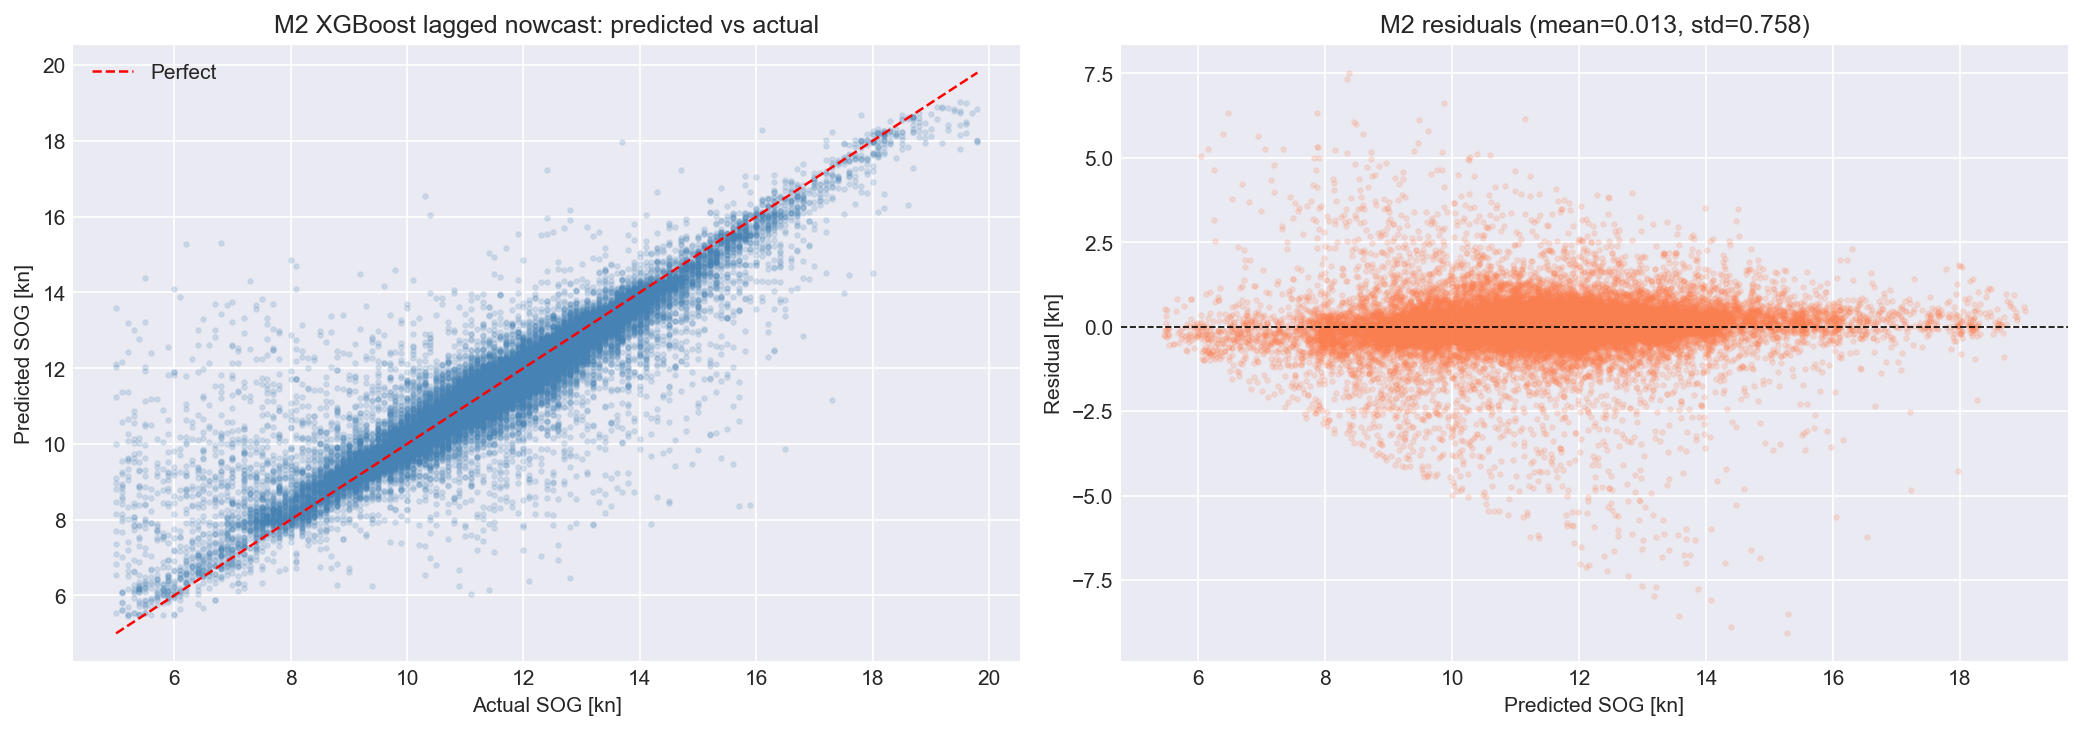
\includegraphics[width=1.0\textwidth]{predicted_vs_actual.png}
    \caption{Predicted versus actual \sog{} for the lagged nowcast model.}
\end{figure}

\subsection{Feature importance}

The weather-only model ranks course and current interaction terms highly, while
the lagged nowcast model is dominated by recent observed speed. This is
consistent with vessel operations: the current speed carries information about
engine setting, traffic, manoeuvring, loading, and other operational factors
that are not explicitly modelled.

\begin{figure}[H]
    \centering
    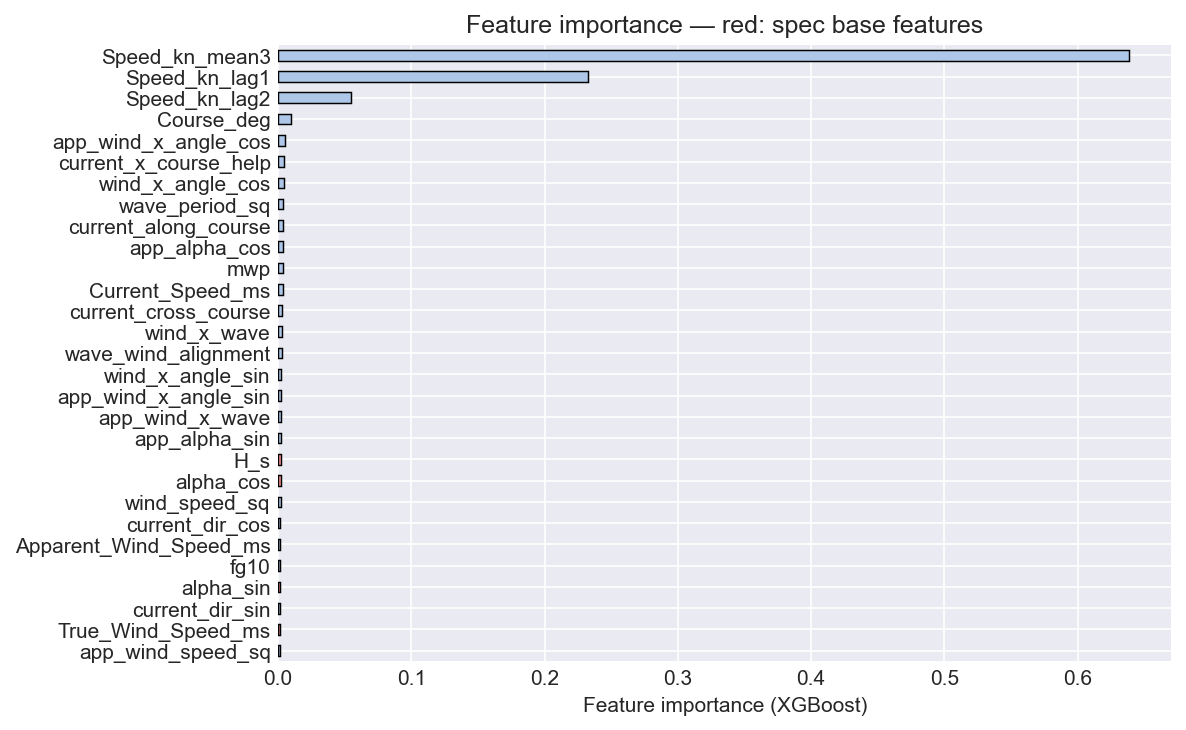
\includegraphics[width=1.0\textwidth]{feature_importance.png}
    \caption{Feature importances for weather-only and lagged nowcast XGBoost
    models.}
\end{figure}

The main interpretation is therefore twofold. First, the project can now predict
short-term \sog{} accurately when recent speed is available. Second, pure
weather-to-speed inference is harder than expected and should be treated as an
explanatory sensitivity tool rather than a final operational predictor.

The feature-importance plot should not be read as a strict physical ranking.
Tree-based importance depends on the model, the correlated features, and the
training distribution. Still, it is useful for checking whether the model is
behaving plausibly. In the weather-only case, route and current-related features
appear alongside wind and wave variables. In the lagged model, recent speed
dominates, which is exactly what we would expect from a nowcast formulation.

One practical interpretation is that future work should not rely only on more
complex models. Additional explanatory variables may matter more than adding
model complexity. Draught, engine power or RPM, loading condition, port
approach flags, and a reliable rotor-operation label could all improve the
ability to separate weather effects from operating decisions.

\section{Rotor and weather-window results}

\subsection{Rotor what-if scenario}

On the test set, the rotor surrogate is active for 35,077 of 35,758 rows, or
98.1\% of observations. The mean rotor power when active is 41.2 \kw{}. The mean
active speed increment is 0.206 \kn{}, and the overall mean increment is
0.202 \kn{}. Per-voyage results are heterogeneous: the highest-gain voyages in
the test set show mean speed contributions from about 0.47 \kn{} to 1.19 \kn{},
while the overall mean remains modest because many observations have weaker
wind, less favourable angle, or low rotor power.

\begin{figure}[H]
    \centering
    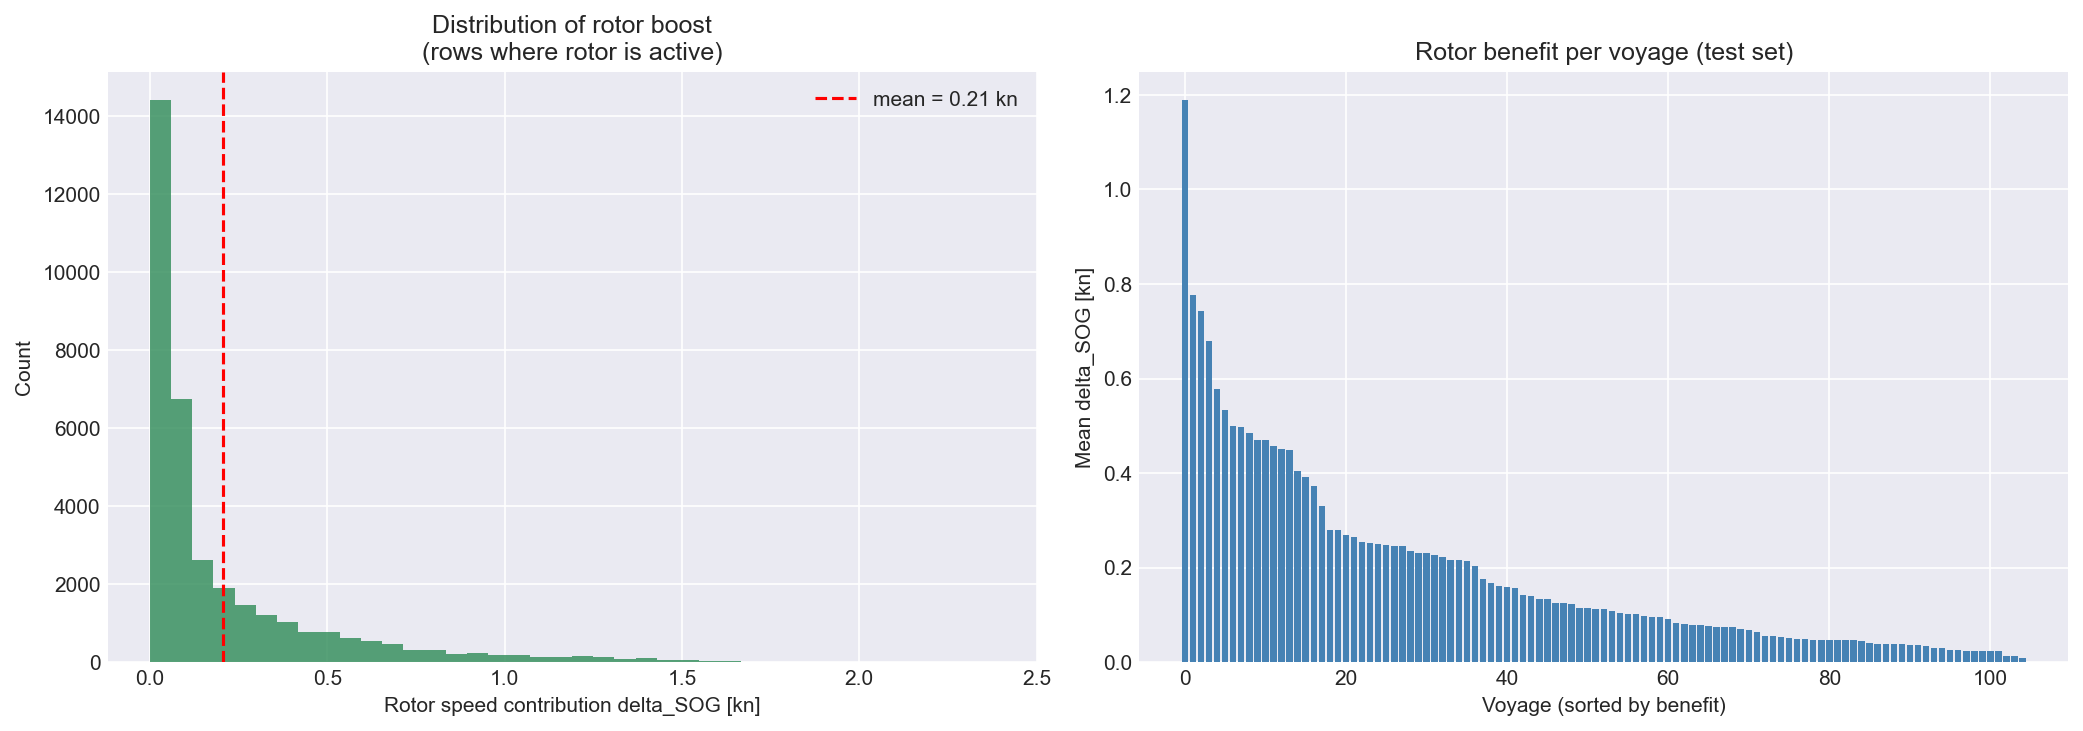
\includegraphics[width=1.0\textwidth]{rotor_scenario.png}
    \caption{Rotor scenario distribution and per-voyage mean speed contribution.}
\end{figure}

The result is operationally meaningful but not spectacular in average speed
terms. An average 0.2 \kn{} speed uplift can still matter over long voyages,
especially if it moves marginal periods over a speed threshold or allows lower
engine load for the same schedule. The larger gains occur in a smaller subset of
conditions, which motivates the gain-detection extension.

The rotor scenario also shows why averages can be misleading. A mean gain of
0.2 \kn{} sounds small, but it is averaged over many different wind angles and
wind speeds. The per-voyage table and gain-detection analysis show that some
voyages experience much larger contributions. For a decision-support tool, this
means the useful question is not only ``what is the average gain?'', but also
``where are the high-gain periods and can we plan around them?''

The active share is high because the implemented gate is permissive: rotor power
only needs to be positive, wave height must be below 6 m, and wind speed must be
below the stop threshold. Active does not mean high impact. It only means the
scenario allows a positive contribution. The high-gain classifier later adds a
more selective view by focusing on observations where the modelled speed
contribution is at least 0.5 \kn{}.

\subsection{Weather-window impact}

The weather-window analysis evaluates whether the rotor scenario helps maintain
the criterion \sog{} $\geq 10$ \kn{} and \hs{} $\leq 3$ m. The result is:

\begin{table}[H]
\centering
\caption{Weather-window comparison on the held-out test set.}
\begin{tabular}{lrrr}
\toprule
\textbf{Scenario} & \textbf{Windows} & \textbf{Points in window} & \textbf{Coverage} \\
\midrule
Baseline prediction & 866 & 27,167 & 76.0\% \\
Baseline + rotor scenario & 808 & 27,696 & 77.5\% \\
Delta & -58 & +529 & +1.5 percentage points \\
\bottomrule
\end{tabular}
\end{table}

The decrease in the number of windows should not be read as a negative result.
When the rotor scenario lifts speed above the threshold between two favourable
periods, separate windows can merge. The more relevant operational result is
that the number of points inside the window increases and total coverage rises.

The window result is best interpreted as a marginal improvement in operational
availability. Coverage rises by 1.5 percentage points on the test set. That is
not a transformation of the whole operating profile, but it is a measurable
change. For a vessel that repeats similar routes many times, small changes in
coverage can accumulate into fewer delays, more schedule flexibility, or lower
fuel use for the same arrival target.

The reduction in the number of windows is a good example of why the project
tracks several indicators. If only the count of windows were reported, the rotor
scenario would look worse. Adding the number of points and coverage shows the
opposite: favourable periods become more continuous. This is exactly the kind of
interpretation that matters when translating model output into maritime
operations.

\subsection{High-gain geography and environmental structure}

The gain-surface and interaction plots show that rotor benefits cluster in
particular wind-speed and angle regimes. This is expected from the polar diagram:
headwind and tailwind directions are poor, while beam and broad-reaching angles
are stronger. Wave height mostly acts as a boundary or risk condition; in the
implemented scenario the rotor is forced off above \hs{} = 6 m, and only 19
observations exceed that threshold in the full engineered dataset.

The gain surface provides the clearest operational message in the rotor
analysis. Rotor benefit is concentrated in a band of wind directions rather than
spread uniformly across all directions. This matches the physical expectation
from the Magnus effect: a rotating cylinder produces a force roughly
perpendicular to the apparent wind, and the useful part of that force depends on
how it projects onto the vessel's direction of travel.

The wave-height interaction is different. Wave height is not the main source of
positive rotor power in this scenario, but it controls whether the scenario is
considered operationally acceptable. In other words, wind angle and speed create
the opportunity, while sea state can remove or limit that opportunity. This
distinction is useful for later route planning because it suggests that a good
rotor route must be both windy in the right way and safe enough in waves.

\begin{figure}[H]
    \centering
    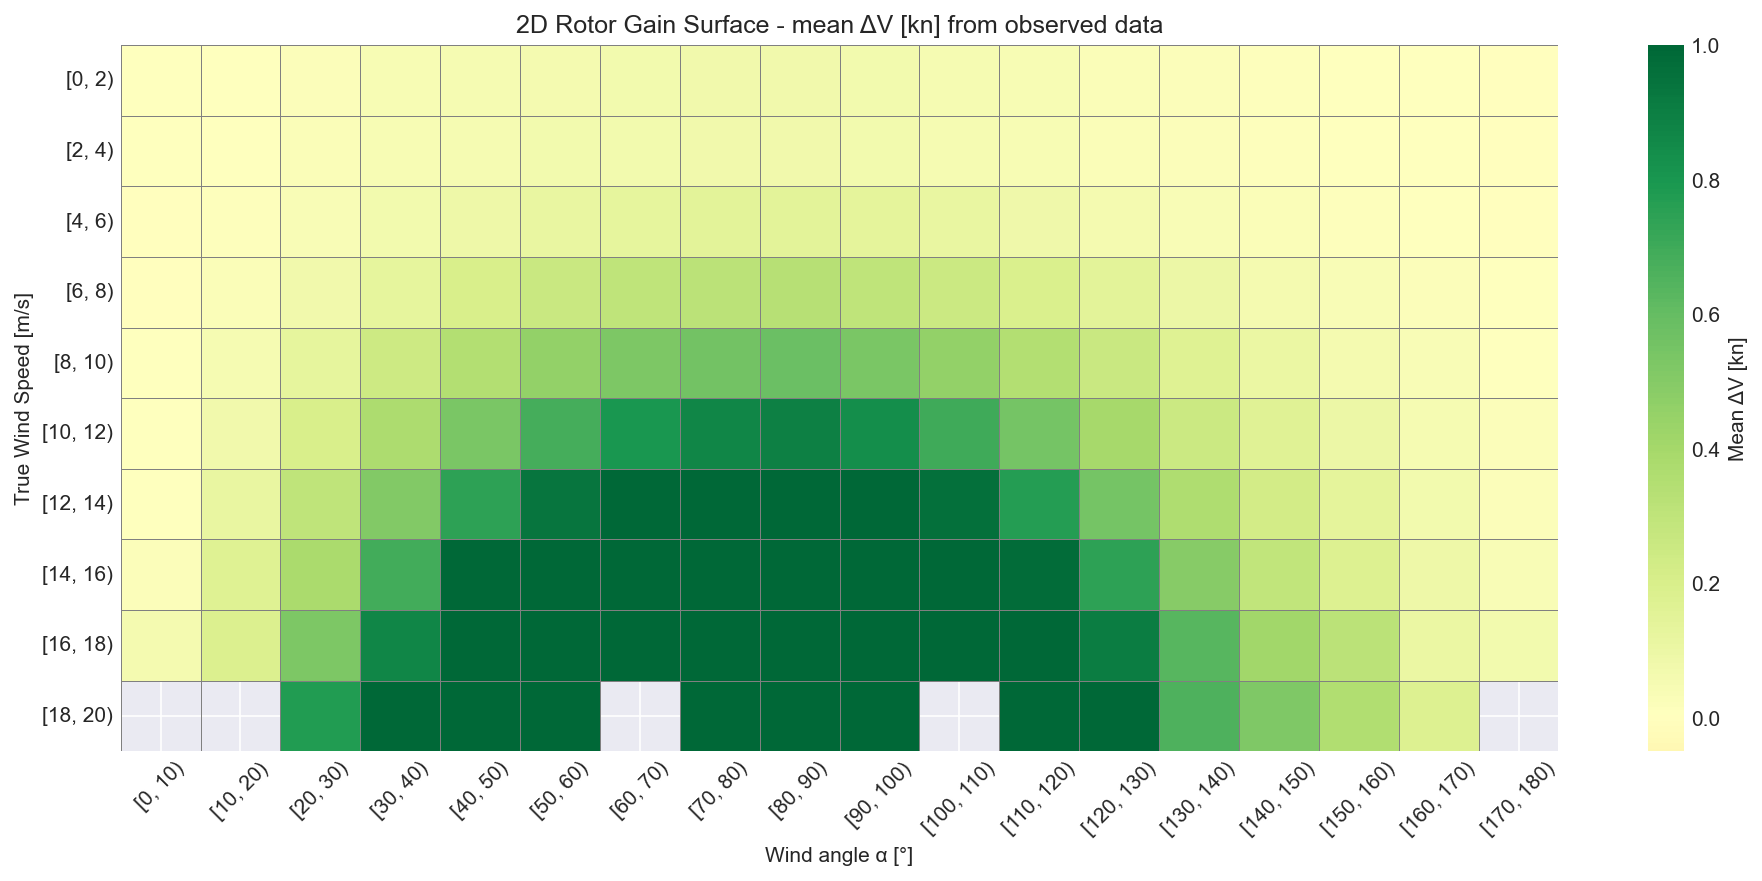
\includegraphics[width=1.0\textwidth]{rotor_gain_surface.png}
    \caption{Environmental structure of the rotor-gain scenario.}
\end{figure}

\section{Energy, emissions, and CII extension}

The first extension converts rotor power into an energy and emissions impact.
The ship model assumes 3,500 \kw{} at design speed 11.5 \kn{}, a cubic
resistance relationship, specific fuel oil consumption of 195 g/kWh, and an HFO
\co{} factor of 3.114 t \co{}/t fuel. Under these assumptions the fuel rate at
design speed without the rotor is 16.38 t/day.

The three-year dataset summary is:

\begin{itemize}
    \item Total observations: 125,160.
    \item Rotor active share: 97.6\%.
    \item Mean brake power: 3,887 \kw{}.
    \item Mean rotor power when active: 40.4 \kw{}.
    \item Total fuel, baseline estimate: 11,066.7 t.
    \item Total fuel, rotor-scenario estimate: 10,954.4 t.
    \item Fuel saved: 112.2 t, or 1.01\%.
    \item \co{} saved: 349.4 t, or 1.01\%.
\end{itemize}

\begin{figure}[H]
    \centering
    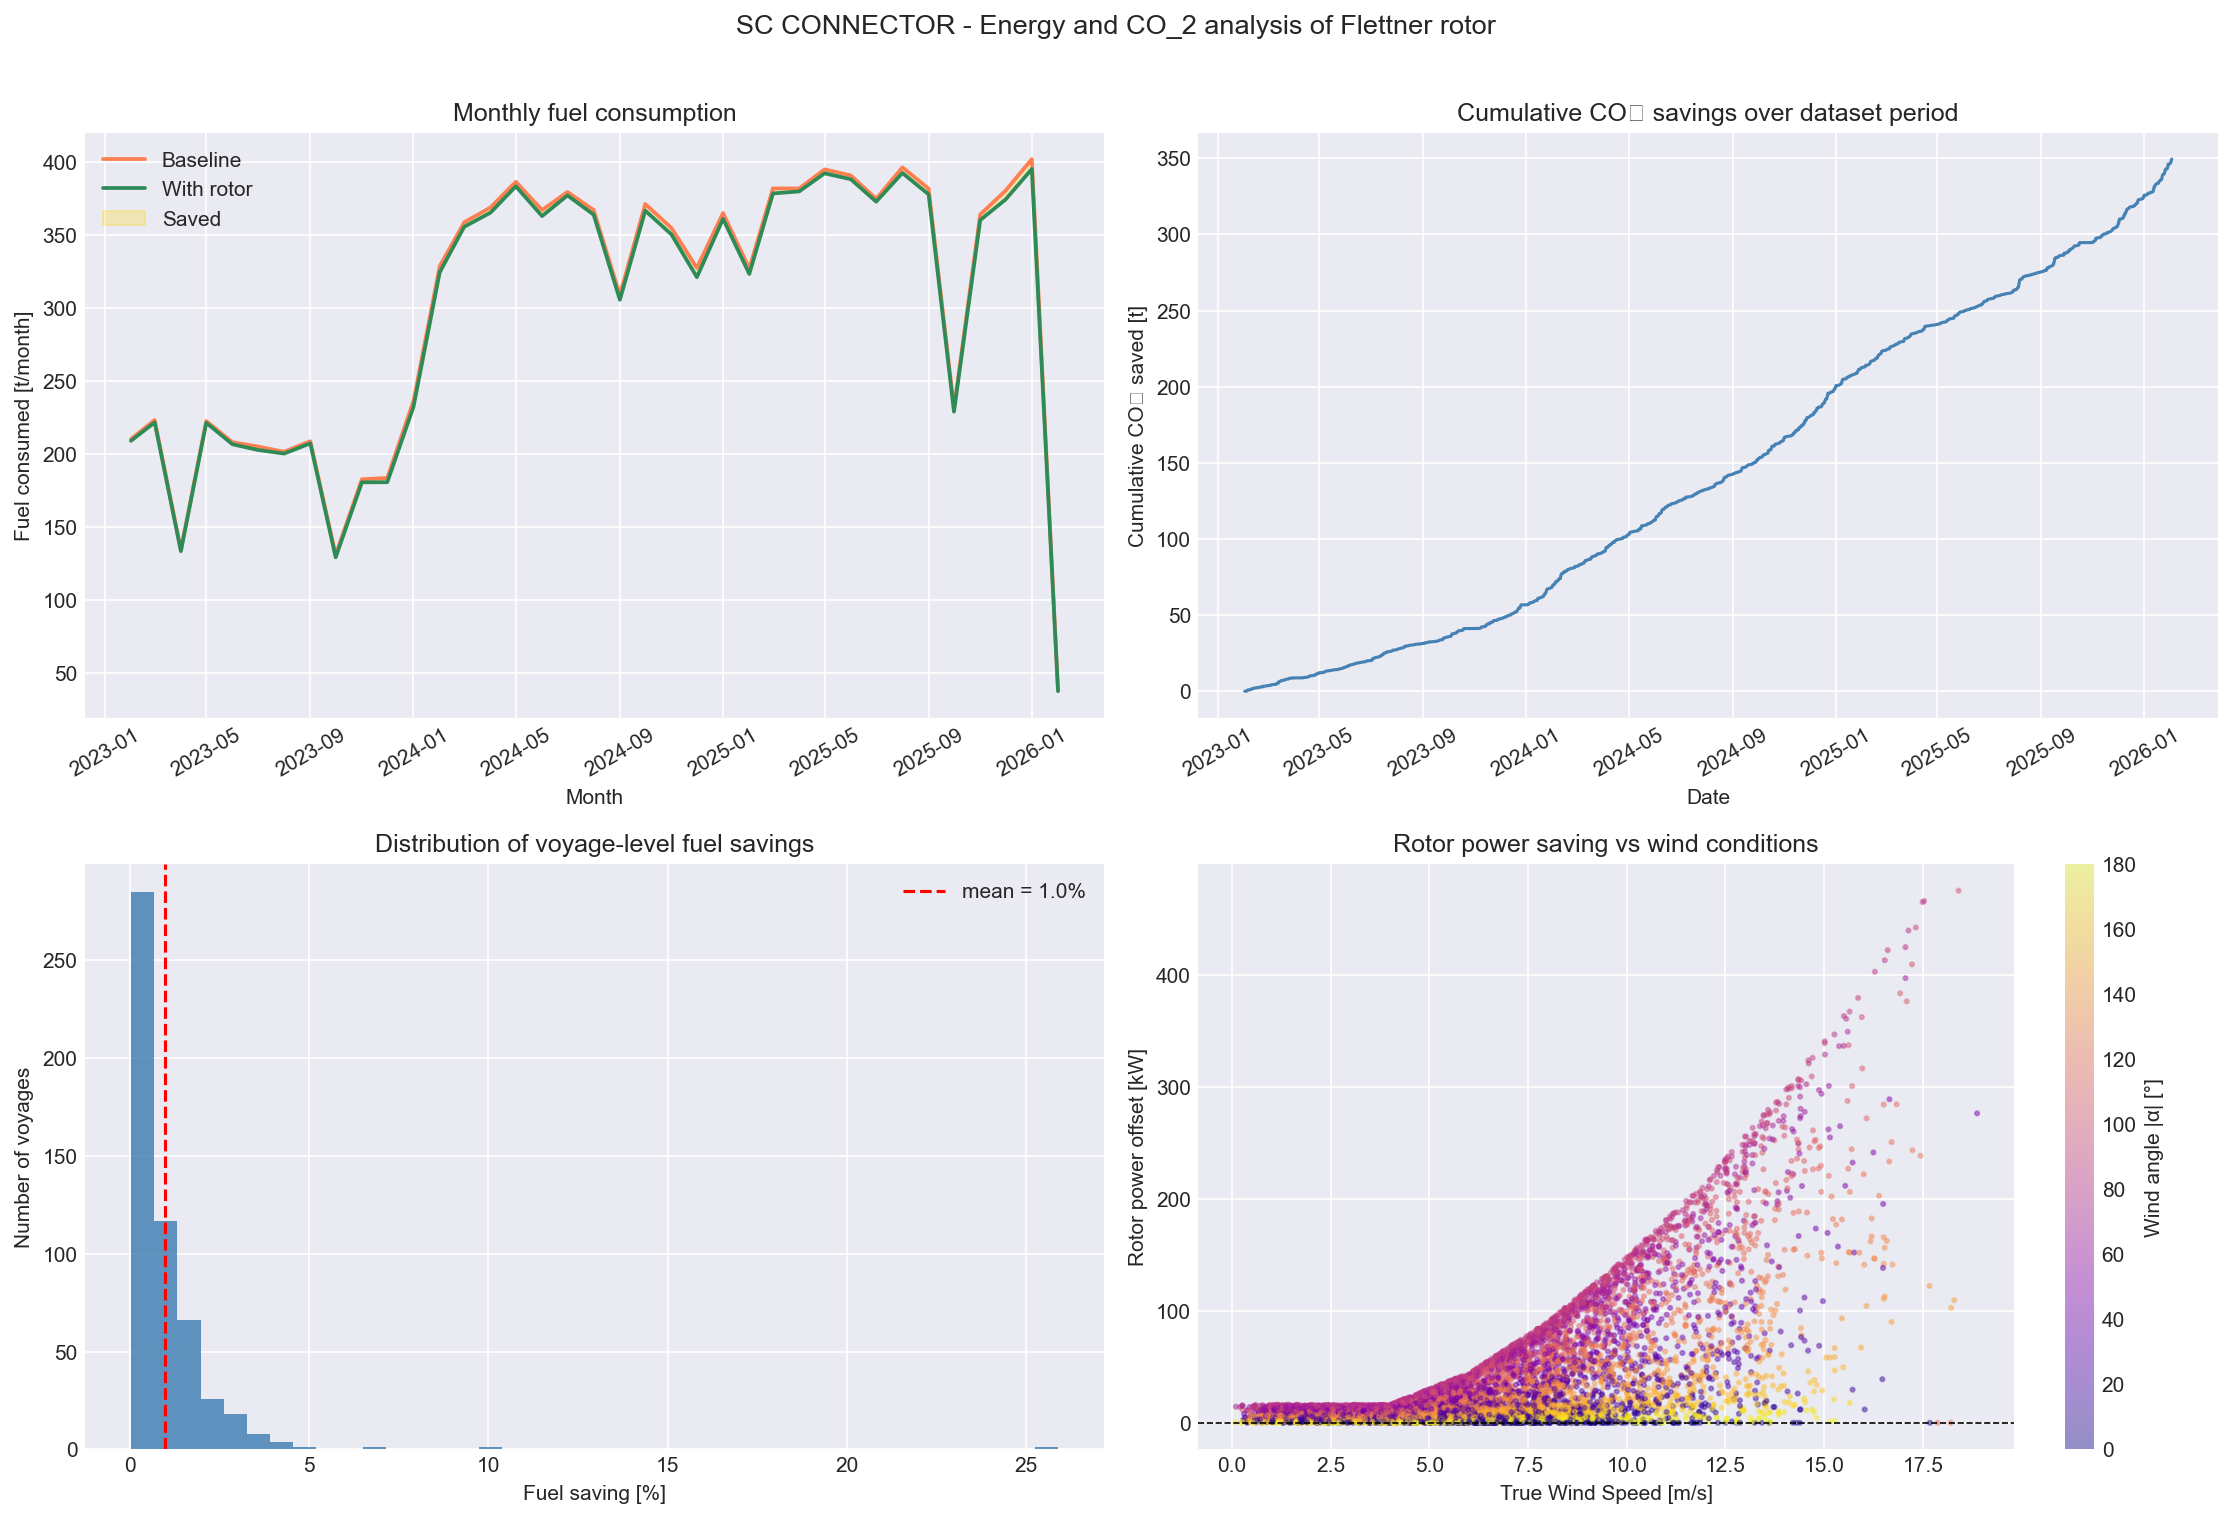
\includegraphics[width=1.0\textwidth]{energy_fuel_co2.png}
    \caption{Fuel and \co{} impact estimated from the rotor energy model.}
\end{figure}

Annualised over the dataset duration of 1,096 days, the extension estimates
37.4 t fuel saved per year and 116.4 t \co{} avoided per year. The attained CII
estimate improves from 53.75 to 53.20 g \co{}/(t nm), a 1.01\% improvement.

The conclusion is that the average annual energy impact is modest for one rotor,
but it is measurable and directionally useful. The result should be interpreted
as an order-of-magnitude scenario rather than a guaranteed vessel-performance
claim, because the historical data do not provide a clean no-rotor control and
the model does not yet include detailed propeller curves, engine load-specific
SFOC, hull fouling, loading condition, RPM control policy, or captain/charterer
speed decisions.

The energy extension is valuable because it translates a speed-oriented rotor
scenario into fuel and emissions language. A small speed increment can be used
in two ways. The operator can keep the same engine setting and arrive slightly
earlier, or reduce engine load and keep approximately the same schedule. The
notebook frames the result as a fuel-saving scenario, which is often the more
important business and environmental interpretation.

The cubic resistance assumption is a standard simplification: required power
increases rapidly with speed. This means that modest speed changes can
correspond to meaningful power differences, especially around normal operating
speed. However, the simplification also means the absolute fuel numbers should
be treated as scenario estimates. The most robust finding is the direction and
order of magnitude of the saving, not an exact guarantee for every voyage.

CII is included because shipping decarbonisation is not only a technical issue
but also a regulatory and reporting issue. Even a roughly one-percent
improvement can be relevant when a vessel is close to a rating boundary or when
operators combine several efficiency measures. The rotor alone is not presented
as a complete decarbonisation solution. It is one operational lever that can
contribute alongside routing, speed management, hull maintenance, and fuel
choice.

\section{Route segmentation extension}

Route segmentation divides the data into heading regimes: northbound,
eastbound, southbound, and westbound. This makes the analysis more interpretable
because rotor performance is strongly tied to the relationship between course
and wind. A single global model can hide differences between legs moving through
different prevailing-wind relationships.

\begin{table}[H]
\centering
\caption{Regime-level characterisation from the full dataset.}
\begin{tabular}{lrrrr}
\toprule
\textbf{Regime} & \textbf{Mean \sog{} [\kn]} & \textbf{Mean wind [\ms]} & \textbf{Mean \hs{} [m]} & \textbf{Mean $\Delta$\sog{} [\kn]} \\
\midrule
Northbound & 12.05 & 7.0 & 1.32 & 0.209 \\
Eastbound & 12.34 & 6.2 & 1.06 & 0.185 \\
Southbound & 10.95 & 6.8 & 1.28 & 0.196 \\
Westbound & 10.58 & 6.5 & 1.21 & 0.209 \\
\bottomrule
\end{tabular}
\end{table}

The per-regime weather-only XGBoost models show mixed predictive quality.
Northbound has the lowest MAE at 1.219 \kn{}, while westbound is hardest to
predict at MAE 1.788 \kn{}. Eastbound is the only regime with clearly positive
$R^2$ in the per-regime model summary, $R^2=0.137$, while the other regimes have
negative $R^2$. This again supports the conclusion that weather-only
generalisation is difficult.

The most useful output from this extension is the weather-window effect by
heading. Westbound legs improve from 85.1\% to 90.1\% coverage, the largest
regime-level gain. Southbound improves from 82.3\% to 84.5\%. Northbound and
eastbound already have high baseline coverage and therefore show smaller
coverage changes.

The regime results show that the same rotor can have different value depending
on route direction. This is expected because a vessel changing heading changes
the relative wind angle even under the same weather system. A northbound leg and
a westbound leg can therefore experience different rotor geometry without any
change in the rotor itself.

The segmentation also helps interpret prediction difficulty. Some regimes are
more regular than others. A route direction with consistent operating patterns
and environmental exposure may be easier to model than a regime that includes
more manoeuvring, port approaches, or mixed conditions. The negative $R^2$
values in several per-regime weather-only models are a warning that splitting
the data does not automatically solve the problem. It improves interpretability,
but each segment still needs enough data and enough explanatory variables.

From an operational perspective, the westbound result is especially interesting
because weather-window coverage changes more strongly there than in the other
regimes. That does not mean westbound is always best for rotors. It means that,
in this dataset and under the chosen threshold, westbound observations contain
more marginal cases that the rotor scenario can move into the acceptable window.

\section{Route optimisation extension}

The route-optimisation extension explores whether route choice can increase the
expected rotor benefit. The implemented proof of concept builds a coarse
0.5-degree spatial grid from historical metocean/rotor-gain fields and applies
Dijkstra search to identify a path with improved integrated rotor gain. The
reference voyage is Voyage 456, from approximately 51.89 degrees N, 4.40
degrees E to 61.23 degrees N, 7.68 degrees E. The great-circle distance is about
570.7 nm.

The spatial field contains 72 grid cells with data. Mean rotor power across the
grid is 78.5 \kw{}, and the best historical cells reach mean rotor powers above
180--290 \kw{} under favourable conditions. The route-search result reports an
optimal path of 19 nodes, distance 568.0 nm versus 571.0 nm for the direct grid
path, mean rotor power 7.5 \kw{} versus 1.9 \kw{} direct, and mean
$\Delta$\sog{} 0.037 \kn{} versus 0.010 \kn{} direct. Relative improvement is
large at +288.5\%, but the absolute gain in this specific route experiment is
small.

\begin{figure}[H]
    \centering
    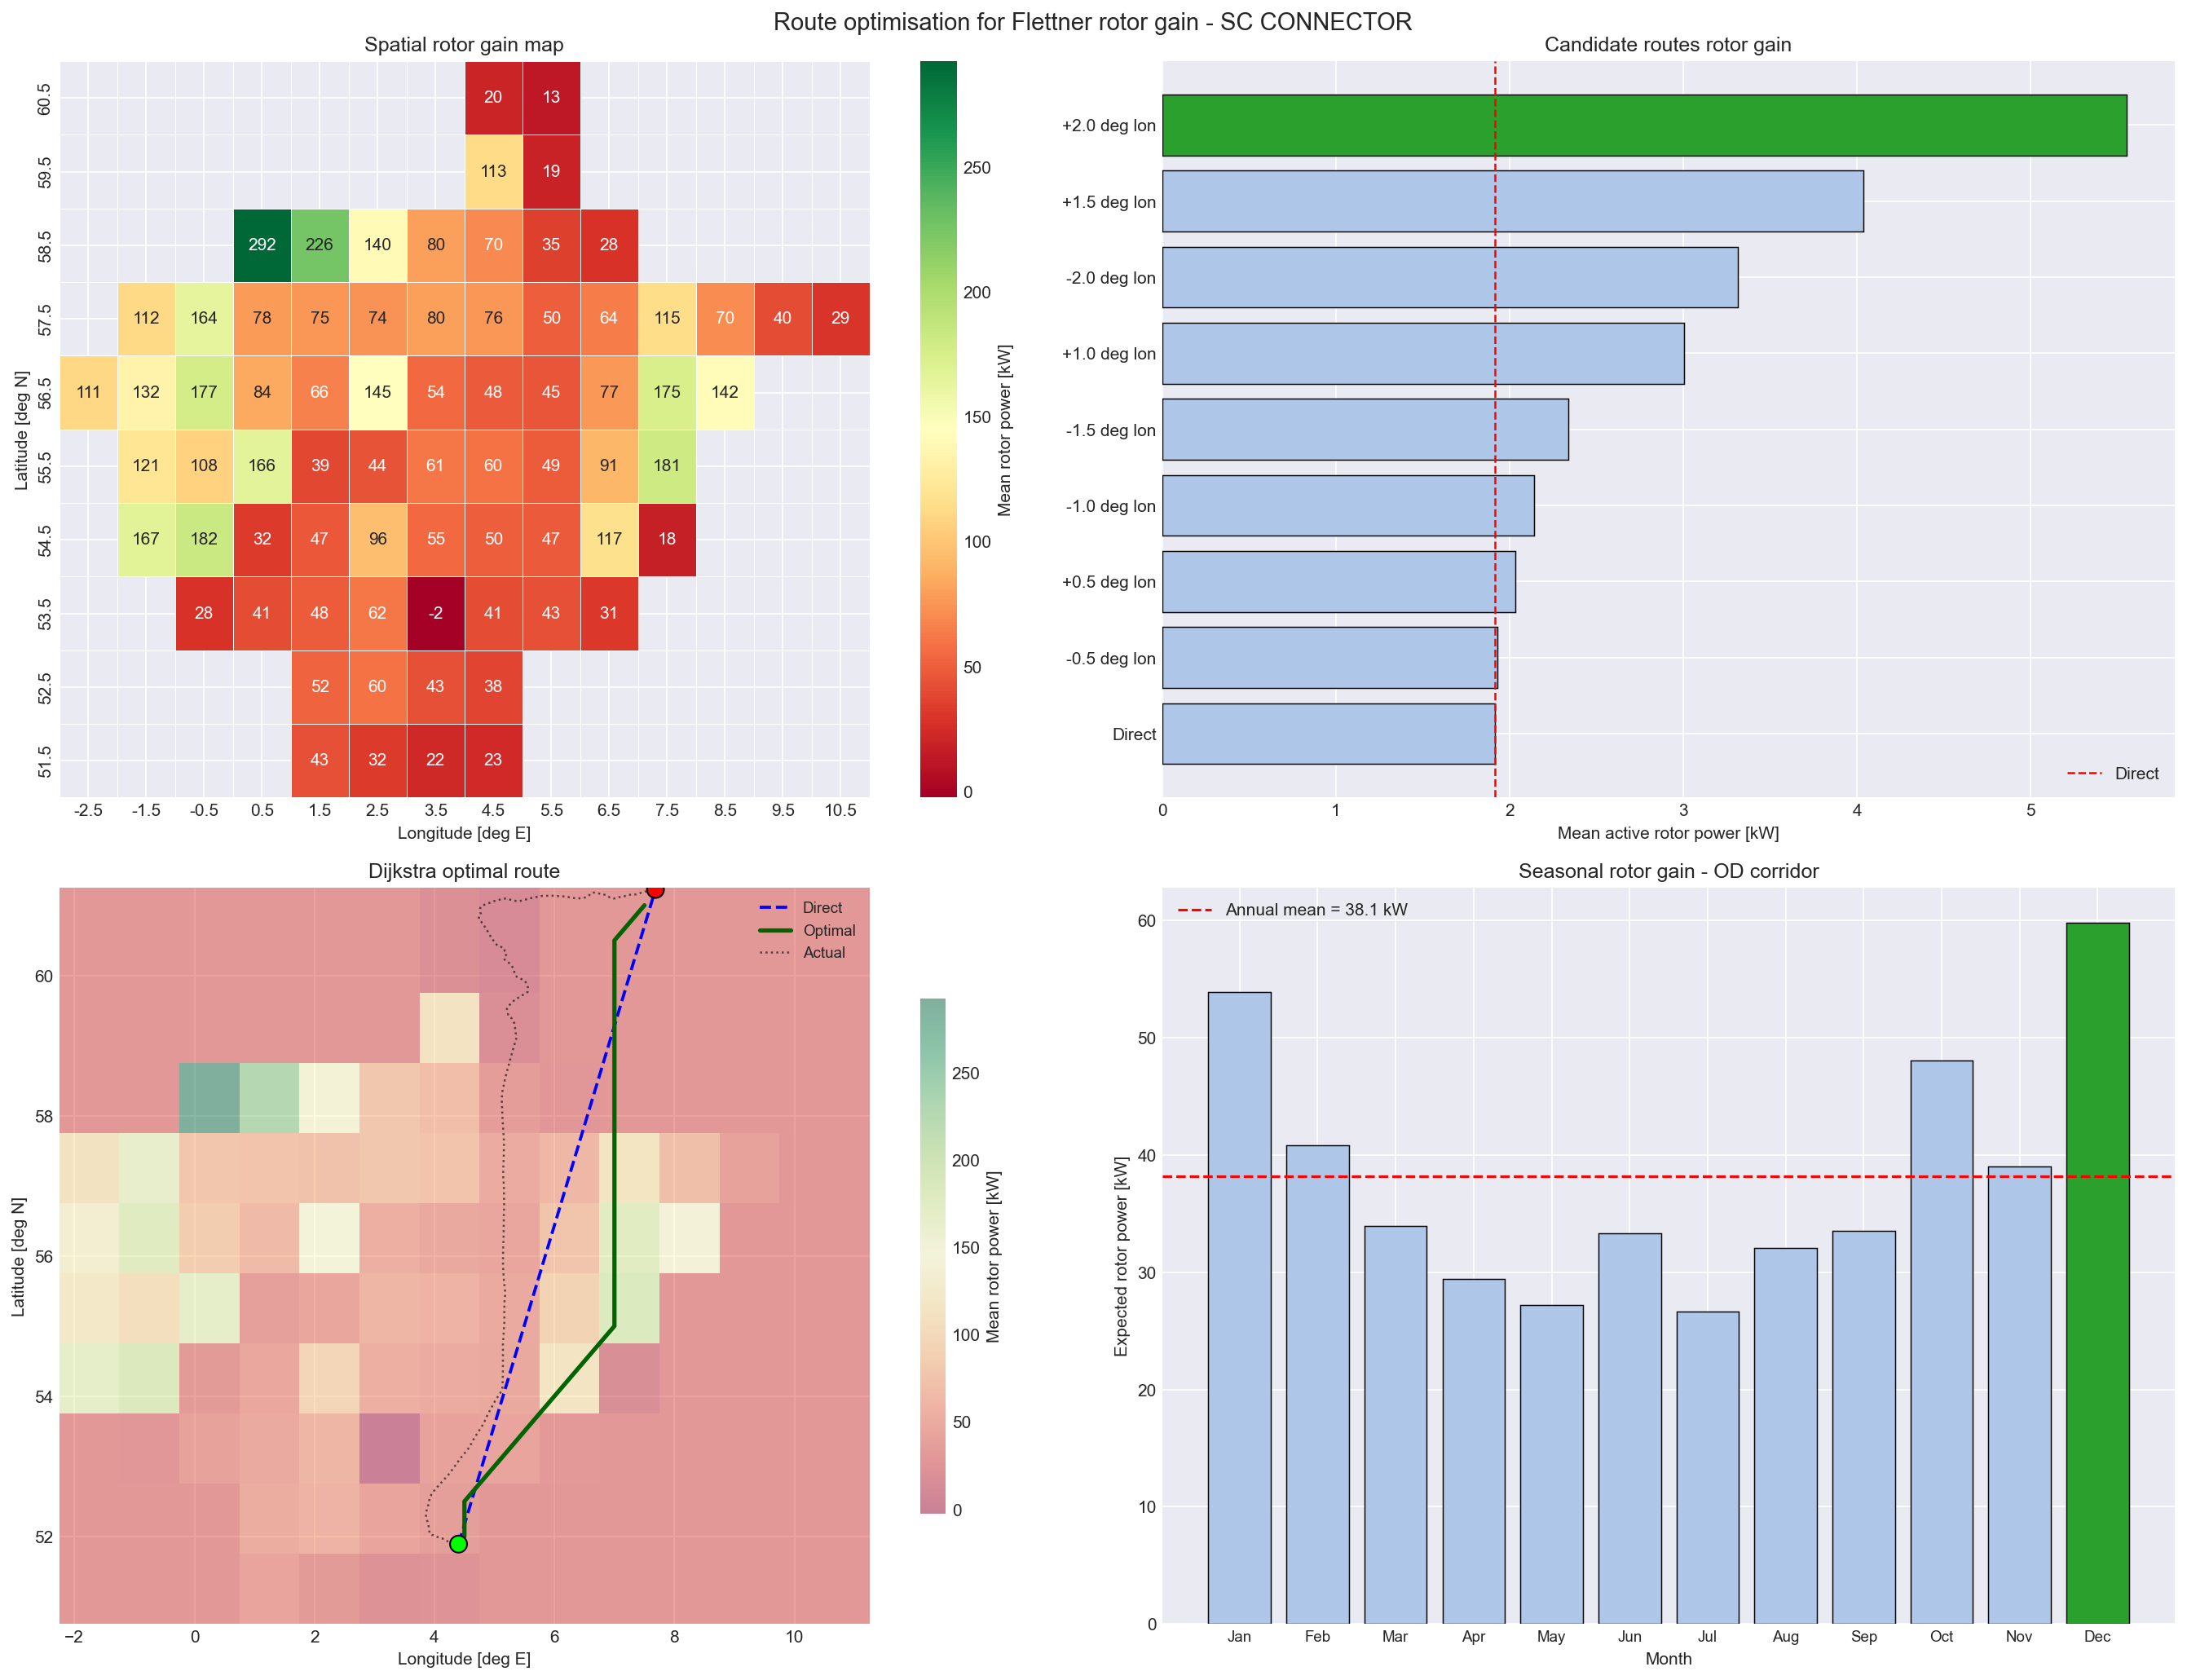
\includegraphics[width=1.0\textwidth]{route_optimization.png}
    \caption{Dijkstra-based routing proof of concept for rotor-gain optimisation.}
\end{figure}

The extension also studies seasonal sensitivity. December has the best expected
monthly rotor power, 59.8 \kw{}, while July is worst at 26.6 \kw{}. The seasonal
pattern is intuitive for the North Sea: winter has stronger winds, but it may
also have more severe waves and operational risk. A final routing product should
therefore optimise a multi-objective score, not rotor gain alone. A practical
score would combine expected arrival time, fuel, \co{}, wave limits, route
deviation, safety margin, and schedule reliability.

The routing extension should be read as a proof of method rather than a final
voyage planner. The current grid is coarse and built from historical fields.
That is enough to show that route geometry can be connected to rotor gain, but a
production routing tool would need forecast fields, land and shallow-water
masks, traffic separation schemes, port constraints, and safety rules.

Dijkstra search is appropriate for a first version because it makes the route
choice explicit. Each grid node and edge can be assigned a cost, and the
algorithm finds the path with the lowest cumulative cost. In this project, the
cost is related to rotor opportunity and route length. In a more complete
version, the edge cost could combine fuel, time, wave risk, distance from the
planned corridor, and uncertainty. The same framework could therefore evolve
from a gain-maximisation example into a multi-objective decision tool.

The seasonal result is also important. The best month for rotor power is not
automatically the best month for operations, because stronger wind can coincide
with higher waves and stricter safety constraints. This reinforces the report's
main theme: rotor benefit is conditional. A good decision-support tool should
not simply search for the strongest wind; it should search for useful wind under
acceptable sea-state and route constraints.

\section{Rotor gain detection extension}

The gain-detection extension turns the rotor scenario into a classification and
decision problem. A high-gain observation is defined as
$\Delta$\sog{} $\geq 0.5$ \kn{}. Under the current surrogate model, high-gain
moments account for 14,856 observations, or 11.9\% of the full dataset.

Rotor gain increases strongly with wind speed. The notebook reports mean
$\Delta$\sog{} of 0.037 \kn{} for wind below 4 \ms{}, 0.273 \kn{} for 8--10
\ms{}, 0.431 \kn{} for 10--12 \ms{}, 0.610 \kn{} for 12--14 \ms{}, and
0.897 \kn{} above 14 \ms{}. The optimal high-gain subset has median wind speed
11.5 \ms{}, and 90\% of those observations are above 9.2 \ms{}.

Angle is equally important. High-gain observations have median absolute relative
wind angle around 82 degrees, with 80\% of the main high-gain subset between 50
and 113 degrees. This matches the rotor polar: beam and quartering winds are
useful, while headwind and tailwind sectors are poor.

\begin{figure}[H]
        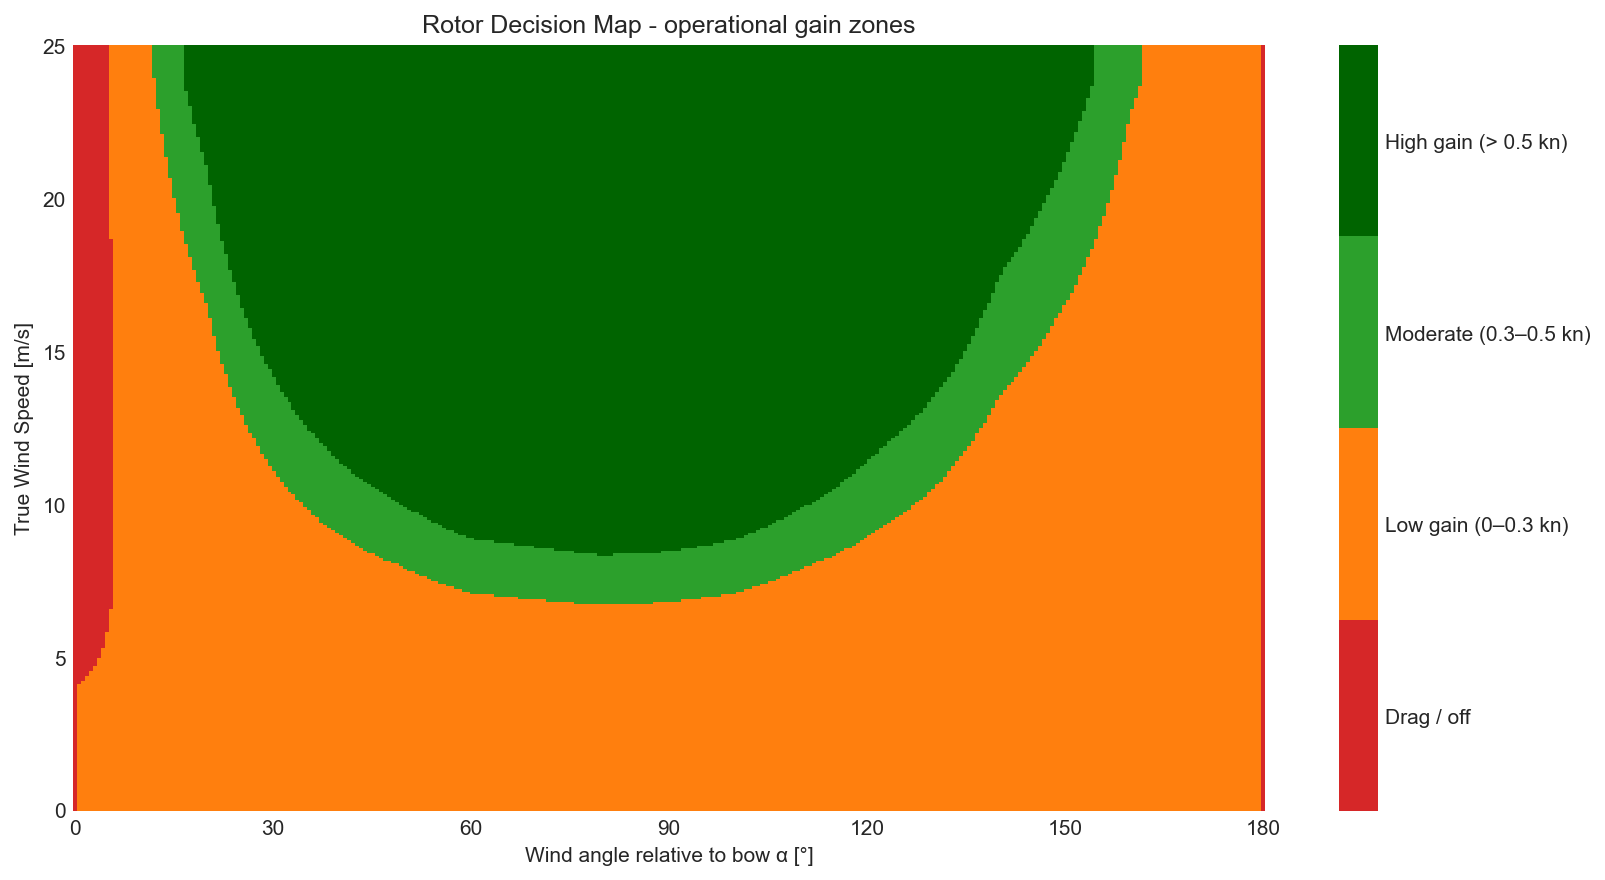
\includegraphics[width=\textwidth]{rotor_decision_map.png}
        \caption{Rule-based high-gain zones.}
\end{figure}

\begin{figure}
        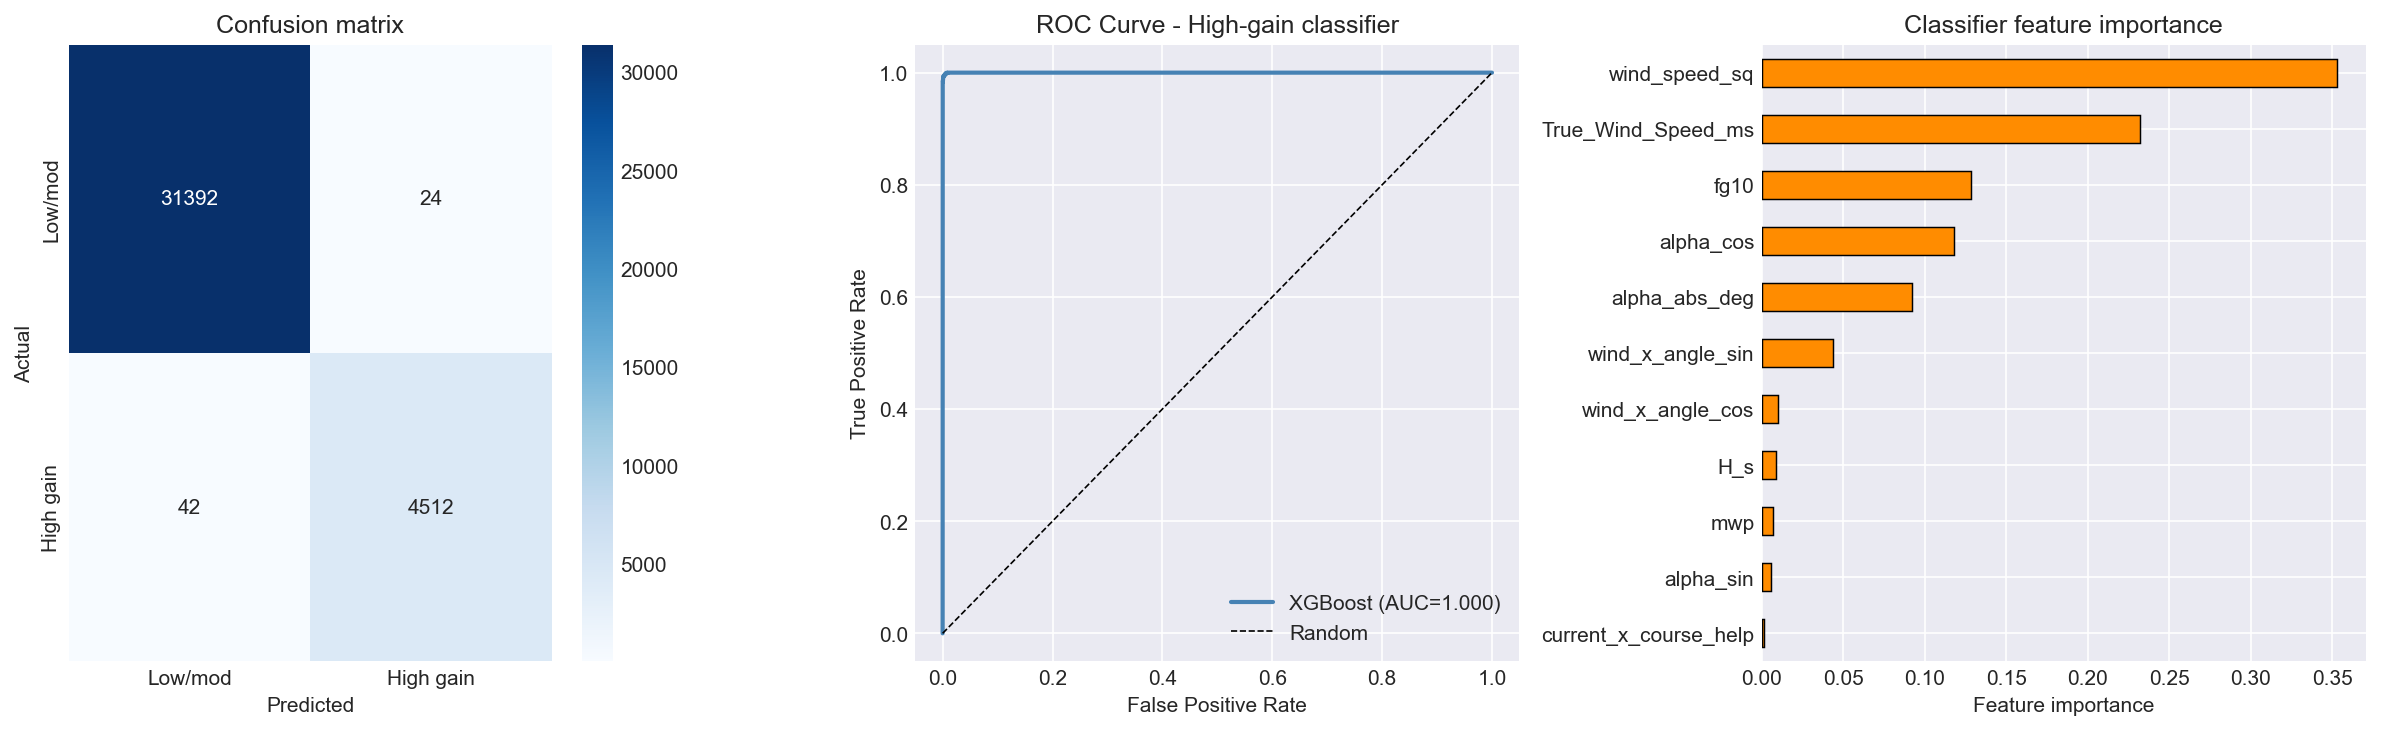
\includegraphics[width=\textwidth]{rotor_classifier.png}
        \caption{Classifier performance.}
\end{figure}
An XGBoost classifier identifies high-gain moments with 99.8\% accuracy,
99.4\% precision, 99.0\% recall, F1 = 0.992, and ROC-AUC = 1.000 on the
notebook split. These very high metrics are plausible because the target is
derived directly from the same rotor-power surrogate and its input variables;
the classifier is therefore best interpreted as a compact decision-rule learner,
not as independent proof of physical rotor performance.

The rule-based decision system is more transparent: if wind is at least 8 \ms{}
and angle is between 50 and 130 degrees, or wind is at least 12 \ms{} and angle
is between 40 and 140 degrees, mark high gain. This rule reaches 95.8\% recall,
69.7\% precision, and 94.2\% accuracy. For operations, the rule is attractive
because it is easy to explain and can be applied to forecasts.

The classifier and the rule-based system serve different purposes. The XGBoost
classifier is accurate because it learns the structure of the model-derived
high-gain label. It is useful as a compact approximation of the scenario model,
but its high score should not be mistaken for independent physical validation.
The transparent rule has lower precision but is easier to communicate: it says
that meaningful rotor moments mostly occur above a wind-speed threshold and
inside a broad favourable angle sector.

This kind of rule is useful for a bridge or operations dashboard. Instead of
showing only a continuous power number, the dashboard can highlight periods as
low, moderate, or high rotor opportunity. A planner can then compare those
periods with route alternatives, schedule constraints, and wave limits. The
result is more actionable than a single annual fuel-saving estimate because it
points to the moments where operational attention matters most.

High-gain detection also helps avoid overclaiming. If only 11.9\% of
observations are high-gain moments, then the rotor's value is concentrated.
This supports a nuanced conclusion: the rotor is not a universal speed boost,
but it can be useful when the environmental geometry is right. That message is
both technically honest and operationally practical.

\section{Implementation notes}

The repository is organised as a reproducible notebook pipeline. The earlier
notebooks prepare and inspect the merged data; the feature-engineering notebook
creates target-safe variables; the baseline model notebook trains and evaluates
the main speed models; the extension notebooks reuse the same feature table for
energy, segmentation, routing, and gain detection. This structure is useful
because it avoids creating separate, inconsistent datasets for each analysis.

The most important implementation choice is that rotor variables are not used as
ordinary model features for the main speed prediction. They are applied after
prediction as a scenario layer. This keeps the baseline model and the
rotor-assisted scenario conceptually separate. If rotor contribution were mixed
directly into the training features without a reliable ON/OFF label, it would be
harder to explain what the model had actually learned.

The notebooks also export figures to the \texttt{results/} directory, which
allows the report to reference a stable set of outputs. This makes the report
less dependent on notebook display state and easier to regenerate. A useful next
engineering step would be to export the most important numerical summaries to a
single compact CSV, so that the report, presentation, and any reviewer checks
all draw from the same result table.

\subsection{Assumptions kept consistent}

The analysis depends on several simplifying assumptions. The most important
point is that these assumptions are used consistently across the notebooks
rather than changed from one extension to another. The rotor polar relationship
is the same scenario utility used for speed uplift, fuel estimation, route
opportunity, and high-gain classification. The voyage-based split is also kept
as the validation principle for the main predictive comparisons. This gives the
project a single analytical spine.

The first assumption is that the merged AIS and metocean table is the common
source of truth. All downstream models use the same temporal and spatial
alignment. This reduces the chance that two notebooks tell different stories
because they were built from slightly different data versions. It also makes
debugging easier: if a result changes, the team can check whether it came from
feature engineering, modelling, or scenario logic.

The second assumption is that the rotor scenario should remain separate from the
baseline speed model. This is a conservative design choice. It avoids training a
model that silently mixes historical vessel behaviour with hypothetical rotor
contribution. It also lets the same baseline prediction be compared before and
after adding the rotor scenario. That makes the difference easier to explain in
the report and presentation.

The third assumption is that the results should be read as decision-support
signals, not as certified performance guarantees. The project uses real
trajectory and environmental data, but it does not yet include the full onboard
instrumentation needed for a formal vessel-performance trial. For a competition
prototype, the useful contribution is the workflow: it shows how to connect AIS,
weather, machine learning, rotor physics, and operational metrics in one
traceable analysis.

These assumptions do not weaken the project if they are stated clearly. On the
contrary, they make the results easier to trust because the reader can see the
boundary between observed data, learned prediction, and simulated rotor effect.
That boundary is important in maritime analytics, where operational decisions
often depend as much on transparent reasoning as on raw model accuracy.

\section{Practical interpretation}

The practical interpretation of the project is that wind-assisted propulsion is
best handled as an operational opportunity map. The rotor benefit depends on
where the vessel is, where it is going, what the wind is doing, and whether sea
state allows the route to remain useful. The project does not claim that one
rotor changes every voyage in the same way. Instead, it identifies the
conditions in which the effect is likely to matter.

For voyage planning, the most useful outputs are the weather-window comparison,
the high-gain decision map, and the route-segmentation results. Together they
answer three practical questions. First, does rotor assistance change the
availability of acceptable operating periods? Second, what wind-speed and angle
zones should the operator look for? Third, which route directions or voyage
segments appear to benefit more under the current data?

For monitoring during a voyage, the lagged nowcast model is more relevant. It
uses recent observed speed and apparent-wind context to predict near-term speed
with much smaller error than weather-only models. That can support alerts when
the vessel is likely to fall below a speed threshold, or when actual performance
differs from what the model expects under the observed conditions.

For emissions reporting, the energy extension provides a bridge from
meteorological opportunity to fuel and \co{} estimates. The exact values depend
on assumptions, but the workflow shows how a rotor scenario can be translated
into quantities that are meaningful for owners, operators, and regulators. This
is important because technical performance is only part of the adoption
question; the business case usually depends on fuel cost, emissions reduction,
schedule reliability, and operational simplicity.

\section{Limitations and next steps}

The main limitation is that the dataset does not fully describe vessel
operation. AIS and metocean data are enough to model observed speed patterns,
but they do not reveal all causes. Engine settings, loading condition, draught,
propeller state, hull fouling, traffic, port manoeuvres, and operator decisions
can all affect \sog{}. Without those variables, the weather-only model has a
limited ceiling.

The rotor scenario is another limitation. It is based on the supplied polar
diagram and a transparent power-to-speed conversion, not on measured onboard
rotor telemetry. Because the historical period may already include rotor use,
the baseline is not a certified no-rotor counterfactual. This is acceptable for
a what-if prototype, but future work should validate the scenario against
measured rotor power, shaft power, fuel flow, or controlled before/after periods
if such data become available.

The route-optimisation extension should also be expanded carefully. Optimising
only for rotor gain can create routes that are not operationally optimal. A
realistic route score should include distance, time, safety, wave exposure,
forecast uncertainty, navigational constraints, and schedule commitments. The
current implementation is valuable because it demonstrates the graph-based
method, but the cost function should become richer before operational use.

The most useful next steps are to export a consolidated results CSV, add
segment-level travel-time error, test several weather-window thresholds, and run
sensitivity checks on the rotor power-to-speed conversion. These additions would
make the project easier to review and would show how stable the main conclusions
are under reasonable changes in assumptions.



\section{Conclusions}

The project has progressed beyond a simple baseline and now forms a coherent
maritime analytics prototype. AIS trajectories are enriched with wind, waves,
and currents; leakage-aware models are trained and evaluated by voyage; rotor
assistance is simulated as a transparent what-if layer; and the results are
translated into weather windows, fuel, emissions, route regimes, routing, and
high-gain operational rules.

The central technical finding is that recent vessel speed is the strongest
predictor of near-term speed. The lagged nowcast model reaches MAE 0.406 \kn{}
and $R^2=0.839$, while weather-only models remain much weaker. This distinction
should be presented honestly: the project can predict speed well in a nowcast
setting, but causal weather-only interpretation is still limited by missing
operational variables.

The central rotor finding is that the average benefit of one rotor is moderate
but operationally relevant. Mean speed uplift is about 0.2 \kn{} across the test
set, weather-window coverage increases by 1.5 percentage points, and the energy
extension gives a scenario estimate of about 37 t/year fuel saving and
116 t/year \co{} reduction. The most useful message is conditionality: the rotor
is most valuable in a minority of high-gain moments, especially when wind is
above roughly 8--12 \ms{} and the apparent wind angle is near beam/quartering
sectors.


\section{Transparency statement}
\label{sec:transparency}

Generative AI tools were used for language polishing, paraphrasing, and
summarisation. The authors performed the analysis, made the modelling and
interpretation decisions, and reviewed the final text for accuracy and
relevance. The tools did not have access to the raw data and did not make
modelling decisions.

\phantomsection
\addcontentsline{toc}{section}{References}
\label{sec:references}

\begin{thebibliography}{9}

\bibitem{imo2020ghg}
International Maritime Organization.
\newblock \textit{Fourth IMO Greenhouse Gas Study 2020}.
\newblock IMO, 2020.
\newblock \url{https://www.imo.org/en/ourwork/environment/pages/fourth-imo-greenhouse-gas-study-2020.aspx}

\bibitem{itu2026ais}
International Telecommunication Union.
\newblock \textit{Recommendation ITU-R M.1371-6: Technical characteristics for VHF automatic identification system using time division multiple access in the maritime mobile service}.
\newblock ITU, 2026.
\newblock \url{https://www.itu.int/rec/R-REC-M.1371}

\bibitem{hersbach2020era5}
H. Hersbach, B. Bell, P. Berrisford, S. Hirahara, A. Horanyi, J. Munoz-Sabater, and others.
\newblock The ERA5 global reanalysis.
\newblock \textit{Quarterly Journal of the Royal Meteorological Society}, 146(730):1999--2049, 2020.
\newblock \url{https://doi.org/10.1002/qj.3803}

\bibitem{copernicusmarine}
Copernicus Marine Service.
\newblock \textit{Copernicus Marine Environment Monitoring Service: marine data and information}.
\newblock European Union Copernicus Programme.
\newblock \url{https://www.copernicus.eu/en/copernicus-services/marine}

\bibitem{traut2014flettner}
M. Traut, P. Gilbert, C. Walsh, A. Bows, A. Filippone, P. Stansby, and R. Wood.
\newblock Propulsive power contribution of a kite and a Flettner rotor on selected shipping routes.
\newblock \textit{Applied Energy}, 113:362--372, 2014.
\newblock \url{https://doi.org/10.1016/j.apenergy.2013.07.026}

\bibitem{lu2020wasp}
R. Lu and J. W. Ringsberg.
\newblock Ship energy performance study of three wind-assisted ship propulsion technologies including a parametric study of the Flettner rotor technology.
\newblock \textit{Ships and Offshore Structures}, 15(3):249--258, 2020.
\newblock \url{https://doi.org/10.1080/17445302.2019.1612544}

\bibitem{xgboost2016}
T. Chen and C. Guestrin.
\newblock XGBoost: A scalable tree boosting system.
\newblock In \textit{Proceedings of the 22nd ACM SIGKDD International Conference on Knowledge Discovery and Data Mining}, 785--794, 2016.
\newblock \url{https://doi.org/10.1145/2939672.2939785}

\bibitem{osm}
OpenStreetMap contributors.
\newblock \textit{OpenStreetMap}.
\newblock \url{https://www.openstreetmap.org/copyright}

\end{thebibliography}

\end{document}
